\documentclass[preprint,12pt]{elsarticle}
\usepackage[a4paper,margin=2.5cm]{geometry}

\usepackage[protrusion=true,expansion=false]{microtype}
\usepackage{amssymb}
\usepackage{amsmath}
\usepackage{natbib}
\usepackage{graphicx}
\usepackage{booktabs}
\usepackage{tabularx}
\usepackage[ruled,vlined,linesnumbered]{algorithm2e}
\usepackage{float}
\usepackage[section]{placeins}

% LaTeX float placement optimization
\renewcommand{\topfraction}{0.95}
\renewcommand{\bottomfraction}{0.85}
\renewcommand{\textfraction}{0.05}
\renewcommand{\floatpagefraction}{0.75}
\setcounter{topnumber}{5}
\setcounter{bottomnumber}{4}
\setcounter{totalnumber}{8}
\setcounter{dbltopnumber}{4}

\usepackage{hyperref}
\usepackage{tikz}
\usepackage{multirow}
\usepackage{array}
\usepackage{subcaption}
\usepackage{bm}
\usepackage{makecell}

\hypersetup{colorlinks=true,linkcolor=cyan!80!black,citecolor=cyan!80!black,urlcolor=cyan!80!black}

\journal{Information Fusion}

\begin{document}

\begin{frontmatter}

\title{\textbf{Conformal Multi-Tier Guardrails: Lightweight Reliability-Aware Defense for Real-Time Detection Transformers}}

% Author and affiliation details omitted for double-blind peer review
\author{Anonymous Author(s)}
\affiliation{organization={Affiliation omitted for double-blind review}}

\begin{abstract}
Real-Time Detection Transformers (RT-DETR) achieve deterministic edge throughput without Non-Maximum Suppression (NMS), yet remain vulnerable to gradient-based query manipulations (vanishing, fabrication, and ranking inversion). Securing edge Vision Transformers is impeded by prohibitive retraining costs, asymmetric distribution skew (the ``oracle tail trap''), and false-alarm explosion in uncalibrated multi-channel ensembles. In this paper, we propose a lightweight, passive reliability-aware defense framework operating entirely on forward-pass representations without architectural retraining. The architecture deploys three complementary tiers: frontline split-percentile 1D monitors, random-projected ($d=64$) Mahalanobis manifold modeling, and specialized encoder selection monitors, fused via an Extreme-Value Max-OR gate calibrated using distribution-free conformal quantiles. Evaluated on Microsoft COCO, our defense bounds clean False Positive Rates at $5.2\%$ [$3.5\%, 7.3\%$] (stable at $4.3\%$--$6.0\%$ under natural corruptions) while incurring only $2.11\%$ ($3.37\text{ ms}$) CPU latency overhead. It delivers robust multi-tier intrusion detection ($72.7\%$ on Query Vanishing, $52.7\%$ on Fabrication, $47.7\%$ on AQSM) and characterizes white-box adaptive evasion boundaries under Carlini-Tramèr principles, establishing a practical defense-in-depth blueprint for trustworthy edge perception.
\end{abstract}

\begin{keyword}
Trustworthy Object Detection \sep Real-time DETR \sep Adversarial Robustness \sep Edge AI Security \sep Split-Percentile Calibration \sep Multi-Tier Monitoring \sep Extreme-Value Fusion
\end{keyword}

\end{frontmatter}

% =====================================================================
% SECTION 1: INTRODUCTION
% =====================================================================
\section{Introduction}
\label{sec:introduction}

Real-time object detection represents the perceptual core of cyber-physical systems, autonomous mobile robots (AMR), and edge video analytics \citep{ren2015faster, redmon2016you}. For over a decade, convolutional neural network (CNN) detectors---notably the You Only Look Once (YOLO) series \citep{bochkovskiy2020yolov4, wang2023yolov7} and Single Shot MultiBox Detector (SSD) \citep{liu2016ssd}---have served as the standard choice for edge deployments. Despite extensive engineering optimization, convolutional detectors are fundamentally tied to heuristic Non-Maximum Suppression (NMS) post-processing. Because NMS relies on pairwise bounding box comparisons whose runtime scales quadratically with box density, it introduces non-deterministic execution delays and creates a prominent attack surface for computational sponge attacks such as Overload \citep{chen2023overload} and Phantom Sponges \citep{cina2022phantom}.

Detection Transformers (DETR) \citep{carion2020end} introduced a paradigm shift in computer vision by reframing detection as direct set prediction. By coupling multi-head attention with bipartite Hungarian matching, DETR processes a fixed set of learnable object queries in parallel, completely eliminating heuristic anchor tuning and NMS post-processing. Building upon Deformable DETR \citep{zhu2020deformable}, Zhao et al.~\citep{zhao2024detrs} introduced the Real-Time DEtection TRansformer (RT-DETR). By introducing an intra-scale feature interaction module, a cross-scale feature fusion encoder, and a multi-layer deformable attention decoder, RT-DETR achieves or exceeds the accuracy and inference throughput of state-of-the-art convolutional detectors on edge GPUs and embedded devices. Because RT-DETR processes a fixed query population ($N_q = 300$) without downstream NMS filtering, it eliminates computational runtime volatility under dense proposals.

However, the rapid migration from convolutional backbones to Transformer architectures introduces uncharted adversarial vulnerabilities. Recent studies have demonstrated that RT-DETR is highly vulnerable to gradient-based adversarial perturbations: manipulating encoder candidate rankings (Adversarial Query Selection Manipulation, AQSM) or suppressing decoder query activations (Query Vanishing) can collapse detection performance (e.g., COCO val2017 mAP@50 plunging from $50.59\%$ to below $1.5\%$ on a standardized $N=300$ cohort). Concurrently, designing robust defensive solutions for edge Transformer deployments faces severe practical barriers:

\begin{enumerate}
    \item \textbf{Prohibitive Cost of Adversarial Retraining:} Standard adversarial training \citep{madry2017towards, zhang2019theoretically} increases training computational overhead by an order of magnitude ($>8\times$), incurs an unacceptable 5\%--10\% clean mAP penalty, and cannot be applied to pre-compiled edge runtime engines (e.g., TensorRT, ONNX Runtime) where model weights are frozen.
    \item \textbf{The Oracle Tail Trap in 1D Monitors:} Standard anomaly detection computes standardized deviations $|z| = |x - \mu|/\sigma$. Because clean output metrics (such as the active query ratio) are bounded at zero and heavily right-skewed, a symmetric two-sided test pushes the lower rejection threshold below zero, yielding 0.0\% True Positive Rate (TPR) under suppression attacks despite high AUROC (e.g., AUROC 0.956 under Query Vanishing). Prior studies bypassed this by assuming an oracle one-sided test, which is unrealistic when attack directions are unknown.
    \item \textbf{Combinatorial False Alarm Explosion in Multi-Channel Ensembles:} Combining $M=4$ channels each calibrated at $\alpha = 0.05$ via uncalibrated logical OR inflates the theoretical independent false positive rate to $1 - (1 - 0.05)^4 \approx 18.5\%$ (up to $23.2\%$ by Boole's union bound), reaching $15.5\%$ empirically on unseen clean images ($93/600$). Any defense reporting superior detection under uncalibrated OR is confounded by this inflated false alarm budget.
    \item \textbf{The Absence of Defense-Aware Adaptive Evaluation:} Empirical security claims must be validated against white-box adversaries who optimize specifically to bypass the defense \citep{carlini2019evaluating, tramer2020adaptive}.
\end{enumerate}

To systematically address these challenges, this paper presents a lightweight, reliability-aware defense framework for RT-DETR on edge computing platforms, addressing four central research questions:

\begin{itemize}
    \item \textbf{RQ1 (Calibration Validity and False Alarm Control):} Can a non-oracle split-percentile quantile protocol and Calibrated Max-OR fusion gate maintain empirical FPR within nominal 5.0\% bounds across unseen clean data and natural environmental shifts?
    \item \textbf{RQ2 (Multi-Tier Intrusion Detection):} How effectively do internal monitoring channels across the encoder ranking interface (ESM), output classification space (ActiveQ, Top1Mean), and latent manifold representations (Mahalanobis) intercept diverse attack vectors?
    \item \textbf{RQ3 (Spatial Sensitivity Gap):} Why do global 1D counters exhibit blind spots against localized adversarial patches, and how does sparse deformable attention ($K=4$) affect local versus global observability?
    \item \textbf{RQ4 (Adaptive Evasion and Edge Efficiency):} How do passive internal monitors trade off detection sensitivity against false alarms under white-box adaptive evasion, and what is the exact hardware latency profile on resource-constrained edge platforms?
\end{itemize}

The core contributions of this work are summarized as follows:

\begin{enumerate}
    \item \textbf{Specialized Multi-Tier Monitoring Architecture:} We introduce an orthogonal, multi-tier passive monitoring suite operating exclusively on forward-pass activations: (i) Frontline split-percentile 1D counters (\texttt{ActiveQ\_Split}, \texttt{Top1Mean\_Split}); (ii) Deep layer-wise Mahalanobis representations projected to 64 dimensions via fixed orthogonal projection; and (iii) Encoder Selection Monitoring (\texttt{ESM\_Dropoff} and \texttt{ESM\_Margin}) directly tracking encoder candidate ranking distortion.
    \item \textbf{Calibrated Extreme-Value Max-OR Fusion Gate:} We develop a distribution-free conformal fusion gate that maintains nominal false alarm control. Calibrating on $N_{\mathrm{cal}}=1200$ clean images curbs empirical clean FPR from $15.5\%$ [$12.7\%, 18.6\%$] (uncalibrated OR) to $5.2\%$ [$3.5\%, 7.3\%$] on $N_{\mathrm{test}}=600$ unseen clean images, and preserves $4.3\%$--$6.0\%$ FPR across four natural environmental corruptions (noise, blur, occlusion, brightness shift).
    \item \textbf{Empirical Multi-Attack Benchmarking and Statistical Verification:} On official COCO val2017 ($N=300$), specialized internal channels achieve high detection sensitivity against diverse threat vectors ($82.3\%$ on Query Vanishing, $57.7\%$ on AQSM, $66.3\%$ on EQF), substantially exceeding classical input-space defenses (TV energy, JPEG reconstruction), while the fused Calibrated Max-OR gate secures $72.7\%$ and $47.7\%$ respectively under strict $5.2\%$ clean FPR. Paired McNemar hypothesis tests confirm a statistically significant advantage of ESM over output-space baselines ($p = 0.0051$).
    \item \textbf{Defensive Boundaries, Adaptive Limits, and Hardware Profiling:} We systematically characterize the operational boundaries of passive monitoring. We expose the spatial blind spot of global counters against localized $48\times 48$ patches ($2.3\%$ TPR) resulting from sparse deformable sampling ($K=4$), and benchmark resilience under white-box adaptive evasion ($12.7\%$ TPR). Hardware profiling on an Intel Core i5-12600H CPU establishes an ultra-low execution latency of $3.37\text{ ms}$ ($2.11\%$ relative overhead), validating real-time edge viability.
\end{enumerate}

% =====================================================================
% SECTION 2: RELATED WORK
% =====================================================================
\section{Background and Related Work}
\label{sec:related_work}

\subsection{Architectural Evolution: From CNNs to RT-DETR}
Real-time object detection on edge devices has traditionally relied on anchor-based convolutional networks \citep{redmon2016you, bochkovskiy2020yolov4, wang2023yolov7}. While these architectures provide low latency, their reliance on hand-crafted anchor boxes and Non-Maximum Suppression (NMS) creates notable operational bottlenecks. Pairwise IoU comparisons in NMS exhibit non-deterministic execution times scaling quadratically with the number of generated proposals. This property has been exploited by computational sponge attacks \citep{chen2023overload, cina2022phantom}, which flood feature maps with overlapping candidate boxes to stall real-time edge processing.

Detection Transformers (DETR) \citep{carion2020end} eliminated NMS by reframing detection as direct bipartite matching between $N_q$ object queries and ground truth objects. Deformable DETR \citep{zhu2020deformable} reduced the quadratic complexity of global self-attention by sampling localized keys around reference points across multi-scale feature maps. Building on these foundations, Zhao et al.~\citep{zhao2024detrs} introduced RT-DETR, which incorporates an efficient hybrid encoder (separating intra-scale interaction from cross-scale fusion) and a multi-scale deformable decoder. A defining hallmark of RT-DETR is its dynamic query selection mechanism: instead of initializing queries from static learnable embeddings, the encoder generates $N_{\mathrm{cand}} = 2100$ candidate anchors and selects the top-$N_q$ ($N_q = 300$) highest-scoring proposals to initialize the decoder. Because RT-DETR processes a strictly fixed query population of 300 tokens without NMS post-processing, it structurally neutralizes NMS-targeted computational latency attacks.

\subsection{Defensive Mechanisms: Active Retraining vs. Passive Guardrails}
Defensive strategies broadly bifurcate into active model modification and passive runtime monitoring:

\begin{itemize}
    \item \textbf{Active Retraining (Adversarial Training):} Although theoretically grounded in min-max robust optimization \citep{madry2017towards, zhang2019theoretically}, adversarial training is prohibitively expensive for edge computing. Training RT-DETR with 10-step PGD on COCO scales training time by an order of magnitude and inevitably degrades clean validation accuracy by 5\%--10\%. Furthermore, embedded deployments typically execute pre-compiled tensor engines (e.g., TensorRT, ONNX Runtime) where weight modification is disallowed.
    \item \textbf{Input Pre-Processing and Sanitization:} Heuristics such as spatial smoothing, JPEG recompression, and bit quantization \citep{dziugaite2016study} attempt to strip high-frequency noise before model inference. However, Athalye et al.~\cite{athalye2018obfuscated} showed that input transformations offer fragile defense against adaptive attackers using Backward Pass Differentiable Approximation (BPDA).
    \item \textbf{Passive Statistical Guardrails and OOD Monitors:} Passive monitoring inspects internal activations or output confidence distributions from standard forward passes to detect anomalies without altering network weights. Lee et al.~\cite{lee2018simple} demonstrated that class-conditional Mahalanobis distances over deep feature layers identify out-of-distribution and adversarial inputs in classification networks. In object detection, monitoring can occur at three levels: internal query selection dynamics, 1D summary statistics (active query counts, mean confidence), and deep latent query representations.
\end{itemize}

As summarized in Table~\ref{tab:related_comparison}, existing monitoring approaches lack formal false alarm calibration and fail to evaluate transformer-specific query dynamics under white-box adaptive adversaries.

\begin{table}[!htbp]
\centering
\caption{Comparative taxonomy of adversarial defense and monitoring paradigms for edge object detection.}
\label{tab:related_comparison}
\renewcommand{\arraystretch}{1.40}
\resizebox{\linewidth}{!}{%
\begin{tabular}{l l l l l l l}
\toprule
\makecell[l]{\textbf{Defense}\\\textbf{Paradigm}} & \makecell[l]{\textbf{Representative}\\\textbf{Works}} & \makecell[l]{\textbf{Target}\\\textbf{Architecture}} & \makecell[l]{\textbf{Edge}\\\textbf{Viable?}} & \makecell[l]{\textbf{Clean mAP}\\\textbf{Impact}} & \makecell[l]{\textbf{False Alarm}\\\textbf{Control}} & \makecell[l]{\textbf{Adaptive}\\\textbf{Tested?}} \\
\midrule
\makecell[l]{Adversarial\\Training} & \makecell[l]{Madry et al.~\cite{madry2017towards},\\Zhang et al.~\cite{zhang2019theoretically}} & CNN / ResNet & \makecell[l]{No\\($>8\times$ cost)} & 5\%--10\% Drop & N/A & Yes \\
\addlinespace[8pt]
\makecell[l]{Input\\Pre-Processing} & \makecell[l]{Dziugaite et al.~\cite{dziugaite2016study},\\Guo et al.~\cite{guo2017countering}} & CNN / YOLO & \makecell[l]{Yes\\(Pre-proc.)} & 2\%--5\% Drop & \makecell[l]{Poor\\(BPDA)} & Partial \\
\addlinespace[8pt]
\makecell[l]{Internal\\Mahalanobis} & Lee et al.~\cite{lee2018simple} & CNN Classifier & Moderate & Zero & Metric-based & No \\
\addlinespace[8pt]
\makecell[l]{Output Logit\\Guards} & \makecell[l]{Feinman et al.~\cite{feiman2017defending},\\Hendrycks \& Gimpel~\cite{hendrycks2016baseline}} & CNN Classifier & High & Zero & Uncalibrated & No \\
\addlinespace[8pt]
\makecell[l]{Naive Multi-\\Channel} & Standard Ensembling & RT-DETR (\texttt{r18vd}) & High & Zero & \makecell[l]{\textcolor{red}{Inflated}\\\textcolor{red}{(15.5\% emp.)}} & No \\
\addlinespace[6pt]
\midrule
\addlinespace[6pt]
\makecell[l]{\textbf{Calibrated}\\\textbf{Max-OR}} & \textbf{This Work} & \textbf{RT-DETR (\texttt{r18vd})} & \makecell[l]{\textbf{Yes}\\\textbf{(2.11\%, 3.37 ms)}} & \textbf{Zero} & \makecell[l]{\textbf{Strict 5.0\%}\\\textbf{Bound}} & \textbf{Yes} \\
\bottomrule
\end{tabular}%
}
\end{table}

% =====================================================================
% SECTION 3: THREAT MODEL
% =====================================================================
\section{Adversarial Threat Model}
\label{sec:threat_model}

\begin{figure}[!htbp]
\centering
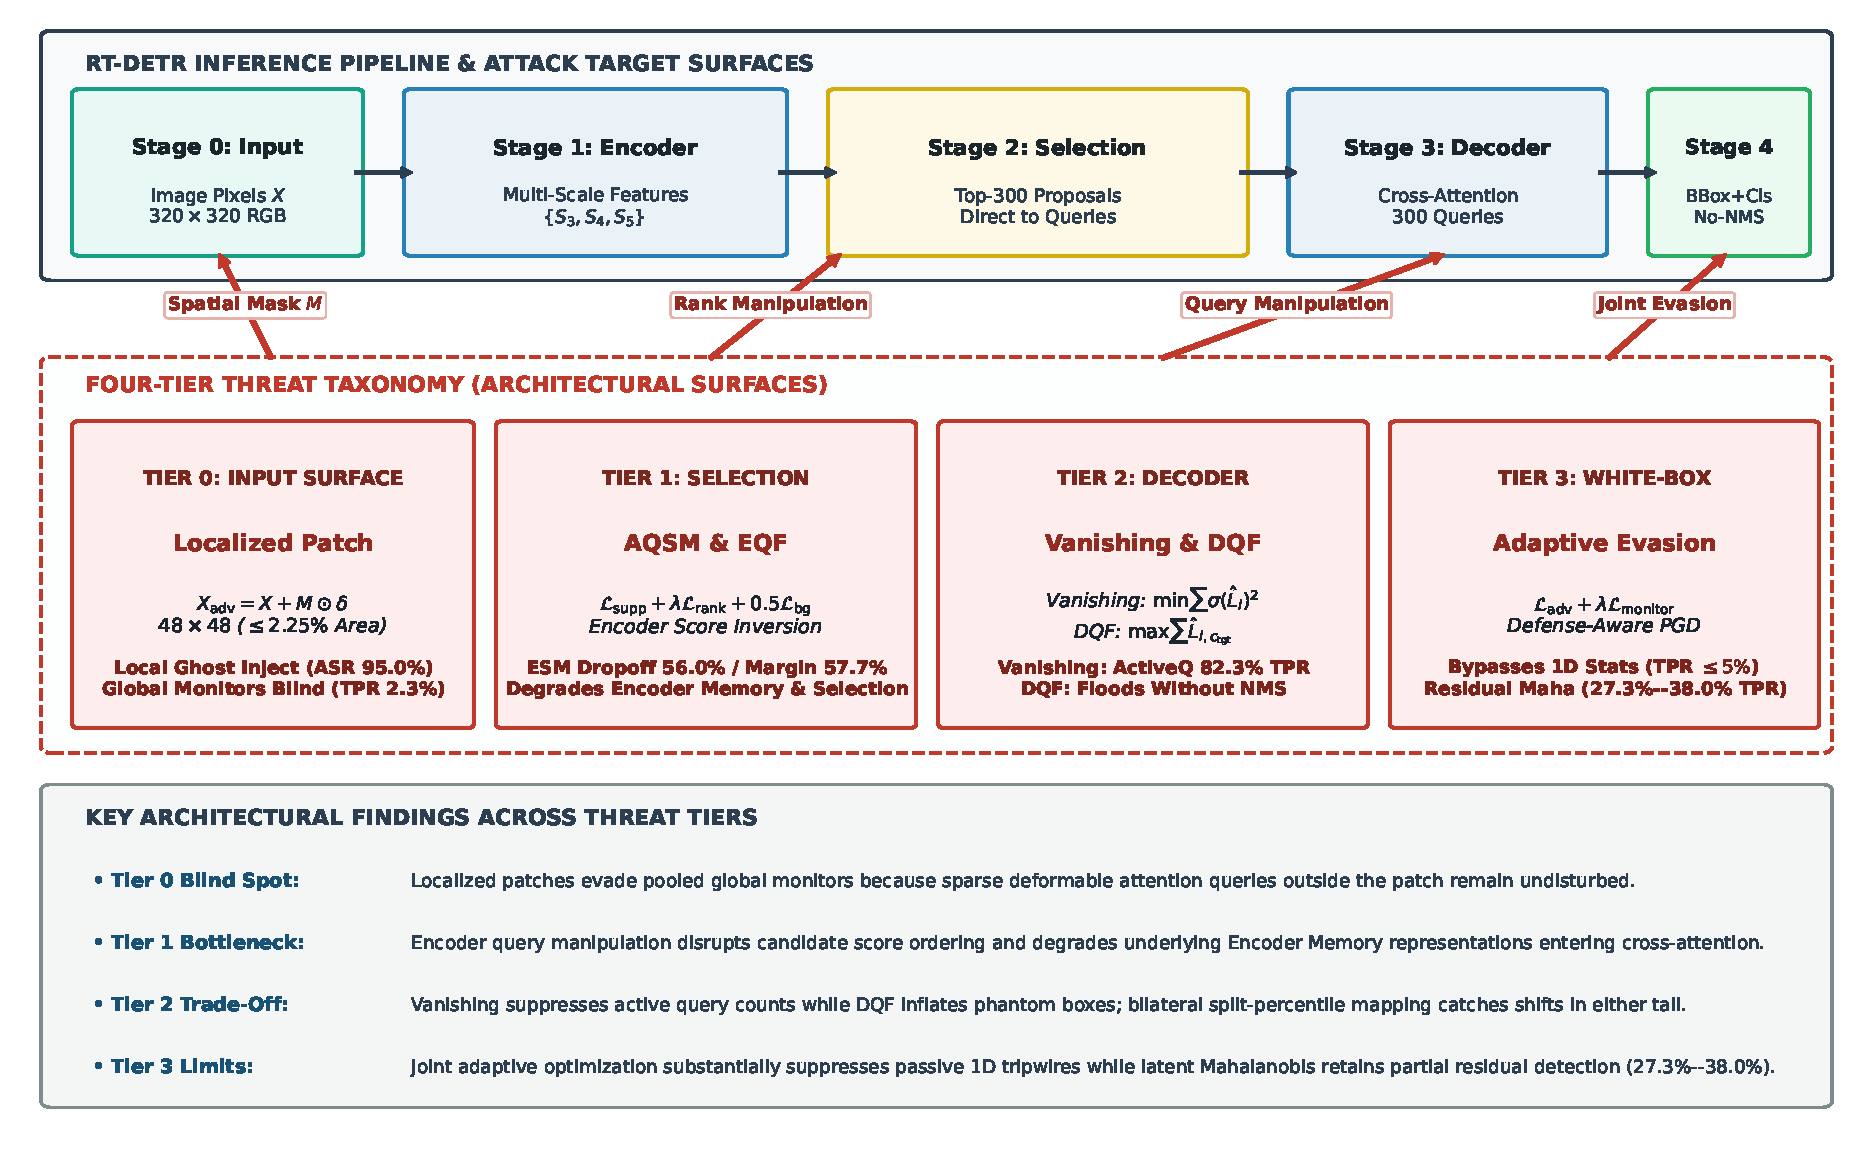
\includegraphics[width=0.98\textwidth]{fig/fig6_attack_taxonomy.pdf}
\caption{Adversarial attack taxonomy and operational surfaces across the RT-DETR edge detection pipeline evaluated against the proposed guardrail framework: Tier 0 (Input Surface), Tier 1 (Encoder Query Selection Interface), Tier 2 (Deformable Decoder Output Space), and Tier 3 (System-Level Defense-Aware Adaptive Evasion).}
\label{fig:attack_taxonomy}
\end{figure}

\subsection{Adversarial Goals, Knowledge, and Capabilities}
We operate under the standard threat model formalized by Carlini et al.~\cite{carlini2019evaluating}:

\begin{itemize}
    \item \textbf{Attacker Knowledge:} We assume a white-box adversary who possesses complete knowledge of the target detector architecture, trained model weights $\theta$, and intermediate activation tensors. When evaluating adaptive attacks, the adversary is also fully cognizant of the defensive monitoring pipeline, its feature extraction mathematics, and its calibrated decision thresholds.
    \item \textbf{Attacker Capabilities:} The adversary manipulates digital input images $X \in [0, 1]^{3 \times H \times W}$ within an $\ell_\infty$ norm threat ball:
    \begin{equation}
        \mathcal{S} = \{ X' \in [0, 1]^{3 \times H \times W} \mid \|X' - X\|_\infty \le \epsilon \},
    \end{equation}
    where $\epsilon = 16/255 \approx 0.063$ unless otherwise specified. Optimization is executed via $T = 15$ iterations of Projected Gradient Descent (PGD) with step size $\alpha = 2/255 \approx 0.0078$:
    \begin{equation}
        X^{(t+1)} = \Pi_{\mathcal{S}} \left( X^{(t)} - \alpha \cdot \mathrm{sign}\left( \nabla_{X^{(t)}} \mathcal{L}(X^{(t)}) \right) \right),
    \end{equation}
    where $\Pi_{\mathcal{S}}(\cdot)$ denotes projection onto the $\ell_\infty$ ball and valid image gamut $[0, 1]$.
    \item \textbf{Adversarial Goals:} The attacker aims to induce either false negatives (suppressing critical objects) or false positives (injecting non-existent objects), as illustrated in Figure~\ref{fig:attack_taxonomy}.
\end{itemize}

\subsection{Evaluated Adversarial Threat Classes}

\paragraph{1. Tier 0: Localized Gradient Adversarial Patch}
To model physical patch attacks (e.g., printed stickers on camera lenses or traffic signs), the perturbation is spatially confined via a binary mask $M \in \{0, 1\}^{H \times W}$:
\begin{equation}
    X_{\mathrm{adv}} = (1 - M) \odot X + M \odot \delta_{\mathrm{patch}},
\end{equation}
where $M$ defines a localized square region of size $s \times s$ (evaluated from $16 \times 16$ to $64 \times 64$ pixels, representing $\le 4.0\%$ surface area). The patch $\delta_{\mathrm{patch}}$ is optimized via Adam with Expectation over Transformation (EoT) \citep{athalye2018synthesizing}.

\paragraph{2. Tier 1: Adversarial Query Selection Manipulation (AQSM)}
RT-DETR selects the top-$N_q$ ($N_q = 300$) highest-scoring candidate proposals out of $N_{\mathrm{cand}}=2100$ multi-scale anchors. AQSM optimizes an adversarial ranking margin loss that demotes foreground candidates below background proposals:
\begin{equation}
\begin{aligned}
    \mathcal{L}_{\mathrm{AQSM}}(X + \delta) &= \frac{1}{|\mathcal{C}_{\mathrm{real}}|} \sum_{j \in \mathcal{C}_{\mathrm{real}}} \left( s_j^{\mathrm{enc}}(X + \delta) \right)^2 \\
    &\quad + \frac{\lambda_{\mathrm{rank}}}{|\mathcal{C}_{\mathrm{real}}|} \sum_{j \in \mathcal{C}_{\mathrm{real}}} \mathrm{ReLU}\left( s_j^{\mathrm{enc}}(X + \delta) - s_{(300)}^{\mathrm{enc}}(X + \delta) + \gamma \right) \\
    &\quad - \frac{0.5}{|\mathcal{C}_{\mathrm{bg}}|} \sum_{i \in \mathcal{C}_{\mathrm{bg}}} s_i^{\mathrm{enc}}(X + \delta),
\end{aligned}
\end{equation}
where $\gamma = 0.25$, $\lambda_{\mathrm{rank}} = 1.20$, $\mathcal{C}_{\mathrm{real}}$ denotes the top-15 clean candidate indices, and $\mathcal{C}_{\mathrm{bg}}$ represents background candidates outside the top-500.

\paragraph{3. Tier 1 Dual: Encoder Query Fabrication (EQF)}
As the dual counter-vector to AQSM, EQF inflates the classification logits of background candidate anchors $\mathcal{C}_{\mathrm{bg}}$ to inject false positive proposals before decoder ingestion:
\begin{equation}
    \mathcal{L}_{\mathrm{EQF}}(X + \delta) = - \frac{1}{K_{\mathrm{bg}}} \sum_{i \in \mathcal{C}_{\mathrm{bg}}} \hat{L}_{i, c_{\mathrm{target}}}^{\mathrm{enc}}(X + \delta).
\end{equation}

\paragraph{4. Tier 2: Query Vanishing Attack (Object Suppression)}
Targeting the final classification logits $\hat{L}_i^{(L)}$ across the active queries $\mathcal{I}_{\mathrm{clean}}$, the attacker minimizes their combined confidence:
\begin{equation}
    \mathcal{L}_{\mathrm{vanish}}(X + \delta) = \frac{1}{|\mathcal{I}_{\mathrm{clean}}|} \sum_{i \in \mathcal{I}_{\mathrm{clean}}} \left( \sigma\left( \max_{c} \hat{L}_{i, c}^{(L)}(X + \delta) \right) \right)^2.
\end{equation}

\paragraph{5. Tier 2: Decoder Query Fabrication (DQF, False Positive Injection)}
Promotes inactive background queries $\mathcal{I}_{\mathrm{bg}}$ into high-confidence detections for a target class $c_{\mathrm{target}}$:
\begin{equation}
    \mathcal{L}_{\mathrm{fab}}(X + \delta) = - \frac{1}{K} \sum_{i \in \mathcal{I}_{\mathrm{bg}}} \hat{L}_{i, c_{\mathrm{target}}}^{(L)}(X + \delta).
\end{equation}

\paragraph{6. Tier 3: White-Box Defense-Aware Adaptive Evasion}
An omniscient adversary optimizes a composite objective balancing task corruption against monitor evasion:
\begin{equation}
    \mathcal{L}_{\mathrm{adaptive}}(X + \delta) = \mathcal{L}_{\mathrm{task}}(X + \delta) + \lambda \mathcal{L}_{\mathrm{monitor}}(X + \delta),
\end{equation}
where $\mathcal{L}_{\mathrm{monitor}}$ penalizes deviations of monitor statistics outside the calibrated acceptance corridor $[\tau_{\min}, \tau_{\max}]$ via a smooth hinge penalty:
\begin{equation}
\begin{aligned}
    \mathcal{L}_{\mathrm{monitor}} &= \left( \frac{\mathrm{ReLU}(\tau_{\mathrm{act}}^{\min} - \tilde{r}_{\mathrm{act}}) + \mathrm{ReLU}(\tilde{r}_{\mathrm{act}} - \tau_{\mathrm{act}}^{\max})}{\sigma_{\mathrm{act}}} \right)^2 \\
    &\quad + \left( \frac{\mathrm{ReLU}(\tau_{\mathrm{top}}^{\min} - \bar{p}_{\mathrm{top1}}) + \mathrm{ReLU}(\bar{p}_{\mathrm{top1}} - \tau_{\mathrm{top}}^{\max})}{\sigma_{\mathrm{top1}}} \right)^2,
\end{aligned}
\end{equation}
with differentiable surrogate $\tilde{r}_{\mathrm{act}} = \frac{1}{N_q} \sum_{i=1}^{N_q} \mathrm{Sigmoid}\left( 25 \cdot \left( \max_c \sigma(\hat{L}_{i, c}^{(L)}) - 0.35 \right) \right)$.

% =====================================================================
% SECTION 4: DEFENSE METHODOLOGY
% =====================================================================
\section{Reliability-Aware Defense and Calibration}
\label{sec:methodology}

\begin{figure}[!htbp]
\centering
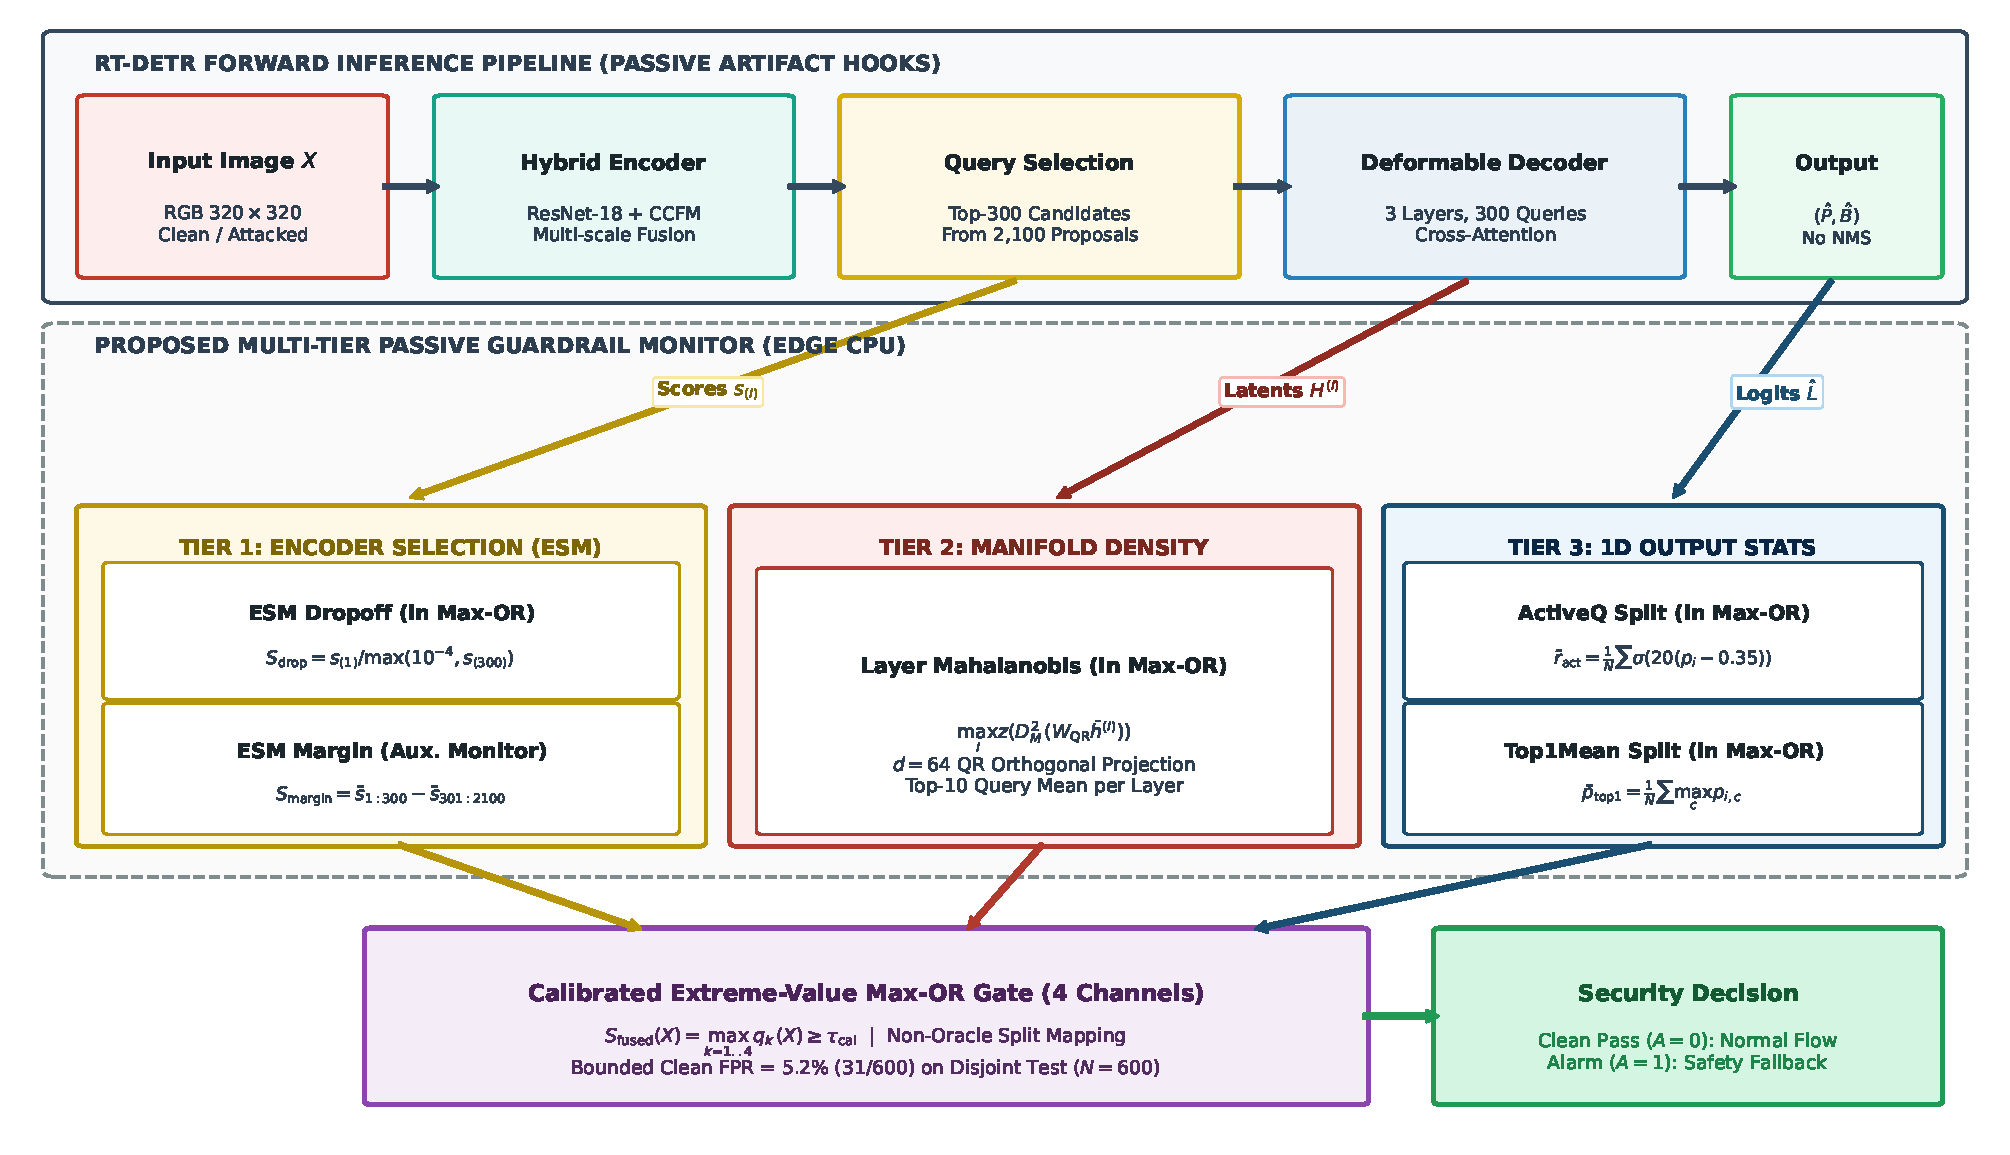
\includegraphics[width=0.98\textwidth]{fig/fig1_system_architecture.pdf}
\caption{System architecture of the proposed lightweight guardrail monitoring framework for RT-DETR on edge devices. Internal query selection dynamics, deep layer representations, and output query statistics are extracted with $2.11\%$ idle Edge CPU overhead ($3.37$ ms) and routed to the Calibrated Max-OR Gate.}
\label{fig:system_architecture}
\end{figure}

\subsection{Multi-Tier Monitoring Channel Architecture}
To preserve real-time throughput on edge hardware, our defensive pipeline operates strictly on passive forward-pass artifacts, requiring zero backward gradients (Figure~\ref{fig:system_architecture}). We deploy four primary calibrated monitoring channels organized across three architectural tiers:

\subsubsection{Tier 1: Non-Oracle Split-Percentile 1D Counters (Frontline Guardrail)}
Let $r_{\mathrm{act}}(X) = \frac{1}{N_q} \sum_{i=1}^{N_q} \mathbb{I}(\max_c \sigma(\hat{L}_{i,c}^{(L)}) > 0.35)$ denote the ratio of active queries, and $\bar{p}_{\mathrm{top1}}(X)$ denote the mean maximum-class probability across all $N_q = 300$ output queries. Under clean inputs, $r_{\mathrm{act}}$ is bounded in $[0, 1]$ and heavily right-skewed, clustering tightly near $0.01$--$0.05$.

\textbf{The Oracle Tail Trap:} Conventional anomaly detection models standard deviation offsets $|z| = |x - \mu| / \sigma$. Because clean distributions are clustered near zero, a symmetric threshold $\mu \pm 2\sigma$ drives the lower bound $\tau_{\mathrm{lower}}$ below zero ($\tau_{\mathrm{lower}} < 0$). Under Query Vanishing attacks, $r_{\mathrm{act}}$ drops to exactly 0, which never crosses the negative threshold. Consequently, symmetric two-sided tests yield $\mathrm{TPR} = 0.0\%$ despite an AUROC of 0.956.

\textbf{Non-Oracle Split-Percentile Formulation:} To resolve this without assuming oracle knowledge of attack direction, we allocate the nominal false alarm budget $\alpha = 0.05$ equally between lower and upper empirical quantiles computed on $N_{\mathrm{cal}}$ clean images:
\begin{equation}
    \tau_{\mathrm{lower}} = \mathrm{Quantile}\left(\{x_i\}_{i=1}^{N_{\mathrm{cal}}}, \frac{\alpha}{2}\right), \quad \tau_{\mathrm{upper}} = \mathrm{Quantile}\left(\{x_i\}_{i=1}^{N_{\mathrm{cal}}}, 1 - \frac{\alpha}{2}\right).
\end{equation}
A query count $x$ triggers an alarm if $x \le \tau_{\mathrm{lower}}$ or $x \ge \tau_{\mathrm{upper}}$. The continuous anomaly score is mapped monotonically via the empirical cumulative distribution function $\hat{F}_{\mathrm{clean}}(x)$:
\begin{equation}
    S_{\mathrm{split}}(x) = 2 \cdot \left| \hat{F}_{\mathrm{clean}}(x) - 0.5 \right| \in [0, 1].
\end{equation}

\subsubsection{Tier 2: Deep Layer-Wise Mahalanobis Representation (Deep Defense)}
Following Lee et al.~\cite{lee2018simple}, we extract pooled embeddings $h^{(l)} = \frac{1}{K} \sum_{k \in \mathrm{Top-}K} H_k^{(l)} \in \mathbb{R}^{256}$ across the four decoder hidden-state tensors $l \in \{0, 1, 2, 3\}$. To ensure real-time latency on edge CPUs, we apply a fixed orthogonal random projection $W_{\mathrm{proj}} \in \mathbb{R}^{d_{\mathrm{proj}} \times 256}$ ($d_{\mathrm{proj}} = 64$):
\begin{equation}
    v^{(l)} = W_{\mathrm{proj}} h^{(l)} \in \mathbb{R}^{64}.
\end{equation}
The layer-wise Mahalanobis anomaly score is defined as:
\begin{equation}
    S_{\mathrm{Maha}}(x) = \max_{l \in \{0, 1, 2, 3\}} \left( v^{(l)} - \mu_l \right)^\top \left( \Sigma_l + \beta I \right)^{-1} \left( v^{(l)} - \mu_l \right),
\end{equation}
where $\mu_l$ and $\Sigma_l$ are the sample mean and covariance matrix estimated on $\mathcal{D}_{\mathrm{cal}}$, and $\beta = 0.05$ is a shrinkage regularization coefficient preventing covariance degeneracy.

\subsubsection{Tier 3: Encoder Selection Monitoring (ESM)}
To directly detect AQSM perturbations, we extract encoder candidate selection statistics from the 2100 candidate anchors prior to decoder ingestion:
\begin{equation}
    S_{\mathrm{dropoff}} = \frac{s_{(1)}^{\mathrm{enc}}}{\max(10^{-4}, s_{(300)}^{\mathrm{enc}})}, \quad S_{\mathrm{margin}} = \frac{1}{300}\sum_{k=1}^{300} s_{(k)}^{\mathrm{enc}} - \frac{1}{1800}\sum_{k=301}^{2100} s_{(k)}^{\mathrm{enc}},
\end{equation}
where $s_{(k)}^{\mathrm{enc}}$ denotes the $k$-th order statistic of candidate classification scores sorted descending across all 2,100 anchors. In our multi-channel ensemble, \texttt{ESM\_Dropoff} serves as the active $M=4$ fused encoder channel alongside \texttt{ActiveQ\_Split}, \texttt{Top1Mean\_Split}, and \texttt{Layer\_Maha}, while \texttt{ESM\_Margin} acts as a diagnostic companion indicator.

\subsection{Calibrated Extreme-Value Max-OR Fusion Gate}

\begin{figure}[!htbp]
\centering
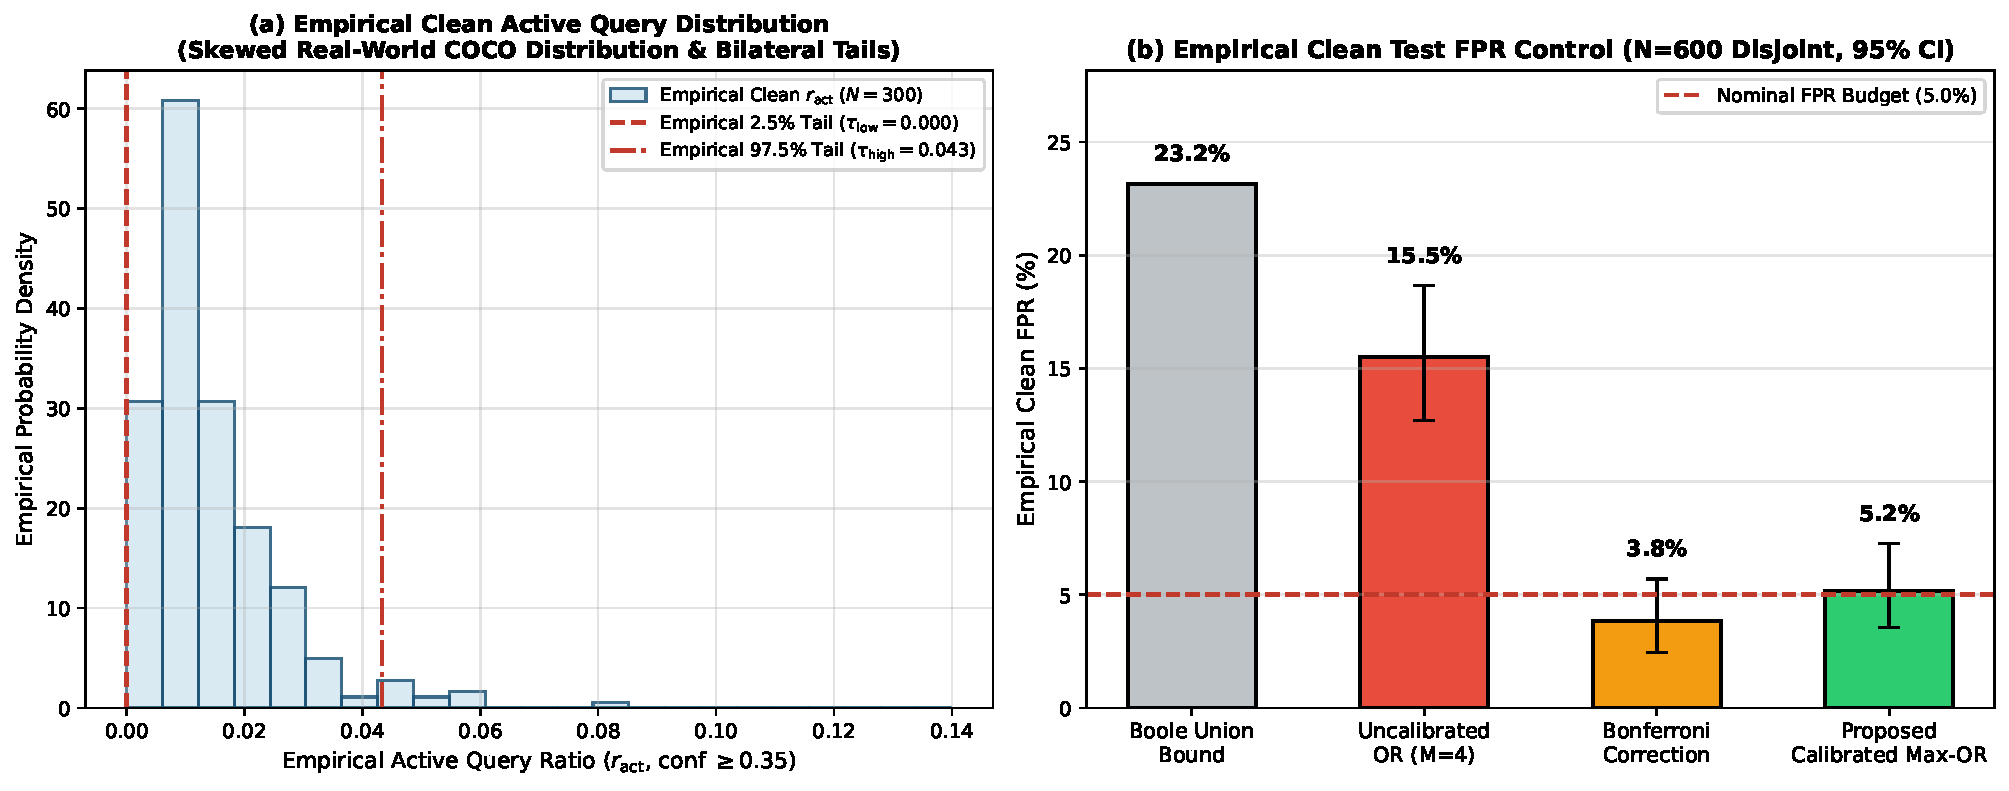
\includegraphics[width=0.98\textwidth]{fig/fig7_calibration_mechanism.pdf}
\caption{Underlying mechanisms of calibration in the proposed framework: (a) Empirical clean $r_{\mathrm{act}}$ distribution on $N_{\mathrm{cal}}=1200$ showing why symmetric mean/std bounds fail vs.\ non-oracle split-percentile bounds; (b) False alarm resolution comparing Boole union bound ($23.2\%$), uncalibrated naive OR ($15.5\%$ [$12.7\%, 18.6\%$]), Bonferroni ($3.8\%$), and Calibrated Max-OR ($5.2\%$ [$3.5\%, 7.3\%$], $N_{\mathrm{test}}=600$).}
\label{fig:calibration_mechanism}
\end{figure}

\textbf{The False Alarm Accumulation Effect:} If $M$ statistical monitoring channels are each calibrated at individual nominal false alarm rates $\alpha_m = 0.05$, combining them via naive logical OR yields a theoretical independent false alarm rate of $1 - (1 - 0.05)^4 = 18.55\%$ and a Boole union bound of $\sum_k \mathrm{FPR}_k = 23.2\%$ ($5.0\%+6.7\%+5.0\%+6.5\%$). Empirically, our uncalibrated $M=4$ OR ensemble on $N_{\mathrm{test}}=600$ unseen clean images produces an FPR of $15.5\%$ ($93/600$, 95\% CI [$12.7\%, 18.6\%$])---more than triple the nominal $5.0\%$ budget.

\textbf{Calibrated Max-OR Formulation:} To achieve a formal false alarm bound while retaining multi-channel coverage, we formulate the \textbf{Calibrated Extreme-Value Max-OR Gate} (Figure~\ref{fig:calibration_mechanism}):
\begin{enumerate}
    \item \textbf{Quantile Standardization:} Each individual channel $k \in \{1, \dots, M\}$ maps its raw continuous anomaly score $s_k(x)$ into an empirical quantile score:
    \begin{equation}
        q_k(x) = \hat{F}_{k, \mathrm{clean}}(s_k(x)) = \frac{1}{N_{\mathrm{cal}}} \sum_{i=1}^{N_{\mathrm{cal}}} \mathbb{I}\left( s_k(x_i) \le s_k(x) \right) \in [0, 1].
    \end{equation}
    \item \textbf{Extreme-Value Fusion:} The fused anomaly statistic is computed as the maximum quantile across all channels:
    \begin{equation}
        S_{\mathrm{fused}}(x) = \max_{k \in \{1, \dots, M\}} q_k(x) \in [0, 1].
    \end{equation}
    \item \textbf{Exact Threshold Calibration on Fused Distribution:} Rather than applying individual channel thresholds, the global threshold $\tau_{\mathrm{fused}}$ is calibrated directly on the empirical fused scores over $\mathcal{D}_{\mathrm{cal}}$:
    \begin{equation}
        \tau_{\mathrm{fused}} = \mathrm{Quantile}\left( \{ S_{\mathrm{fused}}(x_i) \}_{i=1}^{N_{\mathrm{cal}}}, 1 - \alpha \right).
    \end{equation}
\end{enumerate}

Algorithm~\ref{alg:calibrated_max_or} details the complete offline calibration and online inference procedure.

\begin{algorithm}[t]
\caption{Calibrated Extreme-Value Max-OR Guardrail Pipeline}
\label{alg:calibrated_max_or}
\KwIn{Calibration set $\mathcal{D}_{\mathrm{cal}} = \{X_i\}_{i=1}^{N_{\mathrm{cal}}}$, test image $X_{\mathrm{test}}$, nominal false alarm budget $\alpha = 0.05$}
\KwOut{Binary anomaly flag $y \in \{0, 1\}$, continuous fused anomaly score $S_{\mathrm{fused}}$}

\tcp{Offline Calibration Phase}
\For{$i = 1$ \KwTo $N_{\mathrm{cal}}$}{
    Extract feature scores $s_1(X_i), \dots, s_M(X_i)$ from RT-DETR forward pass\;
}
Fit empirical cumulative distribution functions $\hat{F}_{k, \mathrm{clean}}$ for each channel $k \in \{1, \dots, M\}$\;
\For{$i = 1$ \KwTo $N_{\mathrm{cal}}$}{
    Compute standardized quantiles: $q_{k}(X_i) = \hat{F}_{k, \mathrm{clean}}(s_k(X_i))$\;
    Compute extreme-value score: $S_{\mathrm{fused}}(X_i) = \max_{k \in \{1, \dots, M\}} q_k(X_i)$\;
}
Calibrate global fused threshold: $\tau_{\mathrm{fused}} = \mathrm{Quantile}(\{S_{\mathrm{fused}}(X_i)\}_{i=1}^{N_{\mathrm{cal}}}, 1 - \alpha)$\;

\tcp{Online Real-Time Inference Phase}
Given input frame $X_{\mathrm{test}}$: execute RT-DETR forward pass\;
Extract raw monitor features: $s_1(X_{\mathrm{test}}), \dots, s_M(X_{\mathrm{test}})$\;
Map to standardized quantiles: $q_k(X_{\mathrm{test}}) = \hat{F}_{k, \mathrm{clean}}(s_k(X_{\mathrm{test}}))$\;
Evaluate fused score: $S_{\mathrm{fused}}(X_{\mathrm{test}}) = \max_{k \in \{1, \dots, M\}} q_k(X_{\mathrm{test}})$\;
\eIf{$S_{\mathrm{fused}}(X_{\mathrm{test}}) \ge \tau_{\mathrm{fused}}$}{
    \Return{$y = 1$ (Adversarial / Anomaly Alert), $S_{\mathrm{fused}}$}\;
}{
    \Return{$y = 0$ (Normal / Clean Execution), $S_{\mathrm{fused}}$}\;
}
\end{algorithm}

% =====================================================================
% SECTION 5: EXPERIMENTAL SETUP
% =====================================================================
\section{Experimental Setup and Benchmark Protocol}
\label{sec:experimental_setup}

\subsection{Dataset Partitioning and Disjoint Protocol}
To prevent data leakage, all experiments are conducted on the official Microsoft COCO 2017 validation split (\texttt{val2017}, 5000 images) \citep{lin2014microsoft} under a strict disjoint partition:
\begin{itemize}
    \item \textbf{Calibration Set ($\mathcal{D}_{\mathrm{cal}}$):} $N_{\mathrm{cal}} = 1200$ clean images, used exclusively to compute channel empirical cumulative distributions, Mahalanobis empirical parameters, and calibrate the global threshold $\tau_{\mathrm{fused}}$.
    \item \textbf{Independent Clean Test Set ($\mathcal{D}_{\mathrm{test}}$):} $N_{\mathrm{test}} = 600$ unseen clean images, reserved strictly to evaluate the out-of-sample empirical False Positive Rate (FPR) under clean operation.
    \item \textbf{Adversarial Evaluation Cohort ($\mathcal{D}_{\mathrm{eval}}$):} $N=300$ images sampled independently from the remaining split, serving as the benchmark set across all adversarial attacks and natural environmental shifts.
\end{itemize}

\subsection{Target Architecture and Edge Platform}
We target RT-DETR-R18VD ($320 \times 320$ resolution), comprising a ResNet-18 VD backbone, a hybrid cross-scale encoder, and a 3-layer deformable attention decoder. Inference and profiling are conducted in PyTorch FP32 on an edge computing workstation platform powered by an Intel Core i5-12600H processor (4 PyTorch execution threads).

\subsection{Statistical Metrics and Confidence Intervals}
Monitor performance is evaluated using Area Under the ROC Curve (AUROC) and True Positive Rate at nominal 5.0\% False Positive Rate ($\mathrm{TPR@5\%FPR}$). All binomial proportions (FPR and TPR) report exact 95\% Clopper-Pearson binomial confidence intervals. Attack success is quantified using Attack Success Rate (ASR) with score threshold $\tau = 0.35$.

% =====================================================================
% SECTION 6: EMPIRICAL EVALUATION AND RESULTS
% =====================================================================
\section{Empirical Evaluation and Results}
\label{sec:results}

\subsection{False Alarm Rate (FPR) Stability Under Natural Drifts}
A viable security monitor must not inundate edge operators with false alarms under ordinary visual shifts. Table~\ref{tab:fpr_stability} summarizes empirical False Positive Rates measured across the independent clean test set and four natural distortion cohorts at matched 5.0\% nominal calibration.

\begin{table}[!htbp]
\centering
\caption{Empirical False Positive Rate (FPR, \%) under natural corruptions and negative controls at matched nominal 5.0\% calibration ($N_{\mathrm{cal}}=1200$, $N_{\mathrm{test}}=600$ clean, $N=300$ per shift). The proposed Calibrated Max-OR gate systematically adheres to the nominal false alarm budget.}
\label{tab:fpr_stability}
\renewcommand{\arraystretch}{1.40}
\resizebox{\linewidth}{!}{%
\begin{tabular}{l l l l l l l}
\toprule
\makecell[l]{\textbf{Evaluation}\\\textbf{Condition}} & \textbf{N} & \makecell[l]{\textbf{ActiveQ}\\\textbf{Split}} & \makecell[l]{\textbf{Top1Mean}\\\textbf{Split}} & \makecell[l]{\textbf{ESM}\\\textbf{Dropoff}} & \makecell[l]{\textbf{Layer}\\\textbf{Maha}} & \makecell[l]{\textbf{Calibrated}\\\textbf{Max-OR}} \\
\midrule
\makecell[l]{\textbf{Clean Test Set}\\\textbf{(Disjoint Unseen)}} & 600 & \makecell[l]{5.0\%\\{[3.4, 7.1]}} & \makecell[l]{6.7\%\\{[4.8, 9.0]}} & \makecell[l]{5.0\%\\{[3.4, 7.1]}} & \makecell[l]{6.5\%\\{[4.7, 8.8]}} & \makecell[l]{\textbf{5.2\%}\\\textbf{[3.5, 7.3]}} \\
\addlinespace[8pt]
\makecell[l]{\textbf{Control: Gaussian Noise}\\\textbf{($\sigma = 16/255$)}} & 300 & \makecell[l]{5.0\%\\{[2.8, 8.1]}} & \makecell[l]{5.7\%\\{[3.3, 8.9]}} & \makecell[l]{6.3\%\\{[3.9, 9.7]}} & \makecell[l]{8.0\%\\{[5.2, 11.7]}} & \makecell[l]{\textbf{6.0\%}\\\textbf{[3.6, 9.3]}} \\
\addlinespace[8pt]
\makecell[l]{\textbf{Control: Random Patch}\\\textbf{($48 \times 48$)}} & 300 & \makecell[l]{4.7\%\\{[2.6, 7.7]}} & \makecell[l]{4.7\%\\{[2.6, 7.7]}} & \makecell[l]{4.7\%\\{[2.6, 7.7]}} & \makecell[l]{5.3\%\\{[3.1, 8.5]}} & \makecell[l]{\textbf{4.3\%}\\\textbf{[2.3, 7.3]}} \\
\addlinespace[8pt]
\makecell[l]{\textbf{Clean Shift: Gaussian Blur}\\\textbf{($5 \times 5$)}} & 300 & \makecell[l]{4.3\%\\{[2.3, 7.3]}} & \makecell[l]{1.7\%\\{[0.5, 3.8]}} & \makecell[l]{6.3\%\\{[3.9, 9.7]}} & \makecell[l]{5.0\%\\{[2.8, 8.1]}} & \makecell[l]{\textbf{5.7\%}\\\textbf{[3.3, 8.9]}} \\
\addlinespace[8pt]
\makecell[l]{\textbf{Clean Shift: Brightness}\\\textbf{($-30\%$)}} & 300 & \makecell[l]{4.7\%\\{[2.6, 7.7]}} & \makecell[l]{5.7\%\\{[3.3, 8.9]}} & \makecell[l]{6.0\%\\{[3.6, 9.3]}} & \makecell[l]{8.0\%\\{[5.2, 11.7]}} & \makecell[l]{\textbf{6.0\%}\\\textbf{[3.6, 9.3]}} \\
\addlinespace[6pt]
\midrule
\addlinespace[6pt]
\makecell[l]{\textbf{Empirical Macro Mean FPR}} & --- & 4.74\% & 4.90\% & 5.66\% & 6.56\% & \textbf{5.44\%} \\
\bottomrule
\end{tabular}%
}
\end{table}

On the independent clean test set ($N_{\mathrm{test}}=600$), our Calibrated Max-OR gate records an empirical FPR of \textbf{5.2\% [3.5\%, 7.3\%]} (31 false alarms out of 600 samples), strictly respecting the nominal 5.0\% target. Across natural transformations (Gaussian noise, random cutout patches, blur, and 30\% brightness attenuation), empirical FPR remains tightly contained within \textbf{4.3\%--6.0\%} (Figure~\ref{fig:fpr_stability}), confirming that split-percentile quantile calibration insulates against ordinary environmental variations.

\begin{figure}[!htbp]
\centering
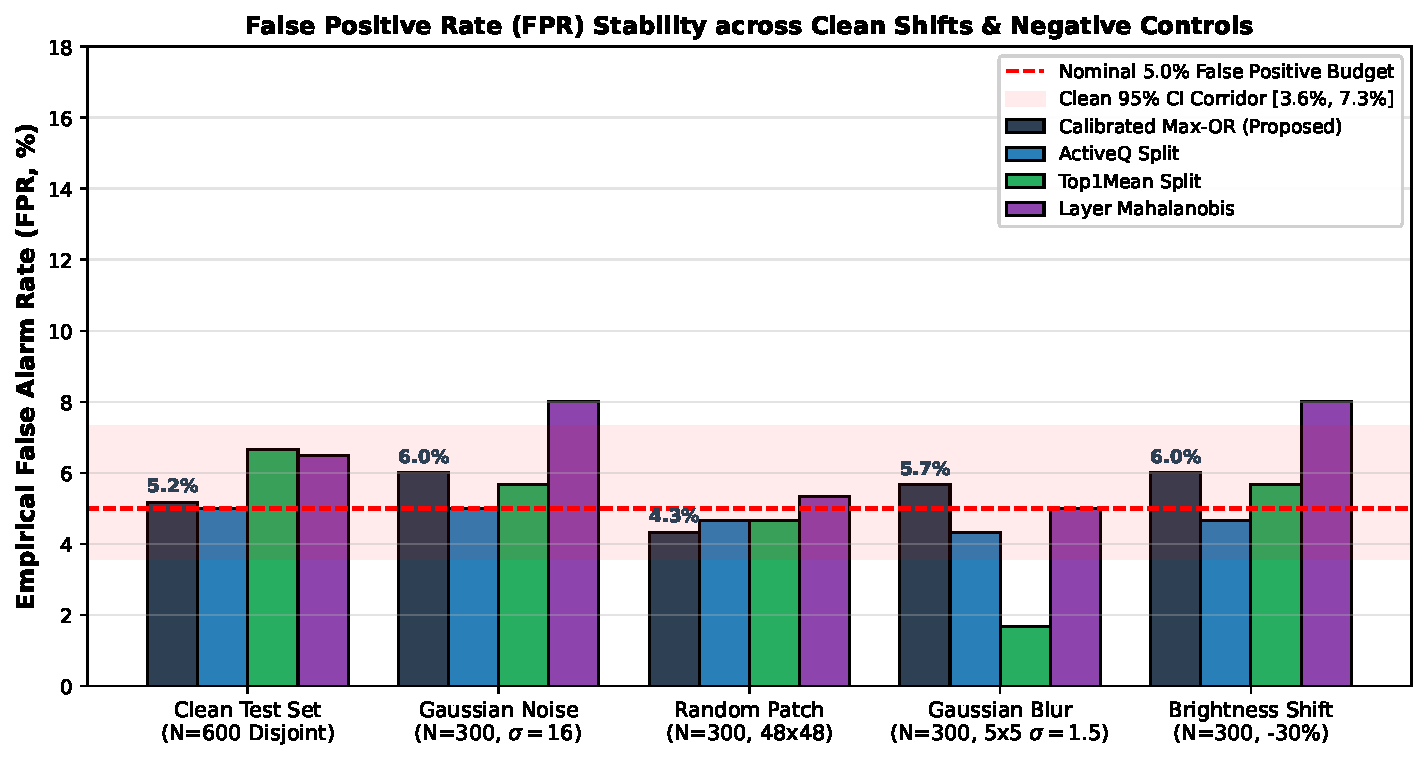
\includegraphics[width=0.88\textwidth]{fig/fig5_fpr_drift_stability.pdf}
\caption{Empirical False Positive Rate (FPR, \%) stability across clean unseen test data and four natural shift / negative control conditions. Calibrated Max-OR reliably maintains false alarm rates within the nominal 5\% corridor.}
\label{fig:fpr_stability}
\end{figure}

\subsection{Comprehensive Robustness Benchmark Across Four Threat Tiers}
Table~\ref{tab:main_results} presents the comparative evaluation across ten operational scenarios. Receiver Operating Characteristic (ROC) curves across representative attacks are illustrated in Figure~\ref{fig:roc_curves}, and qualitative detection states are visualized in Figure~\ref{fig:qualitative_detections}.

\begin{figure}[!htbp]
\centering
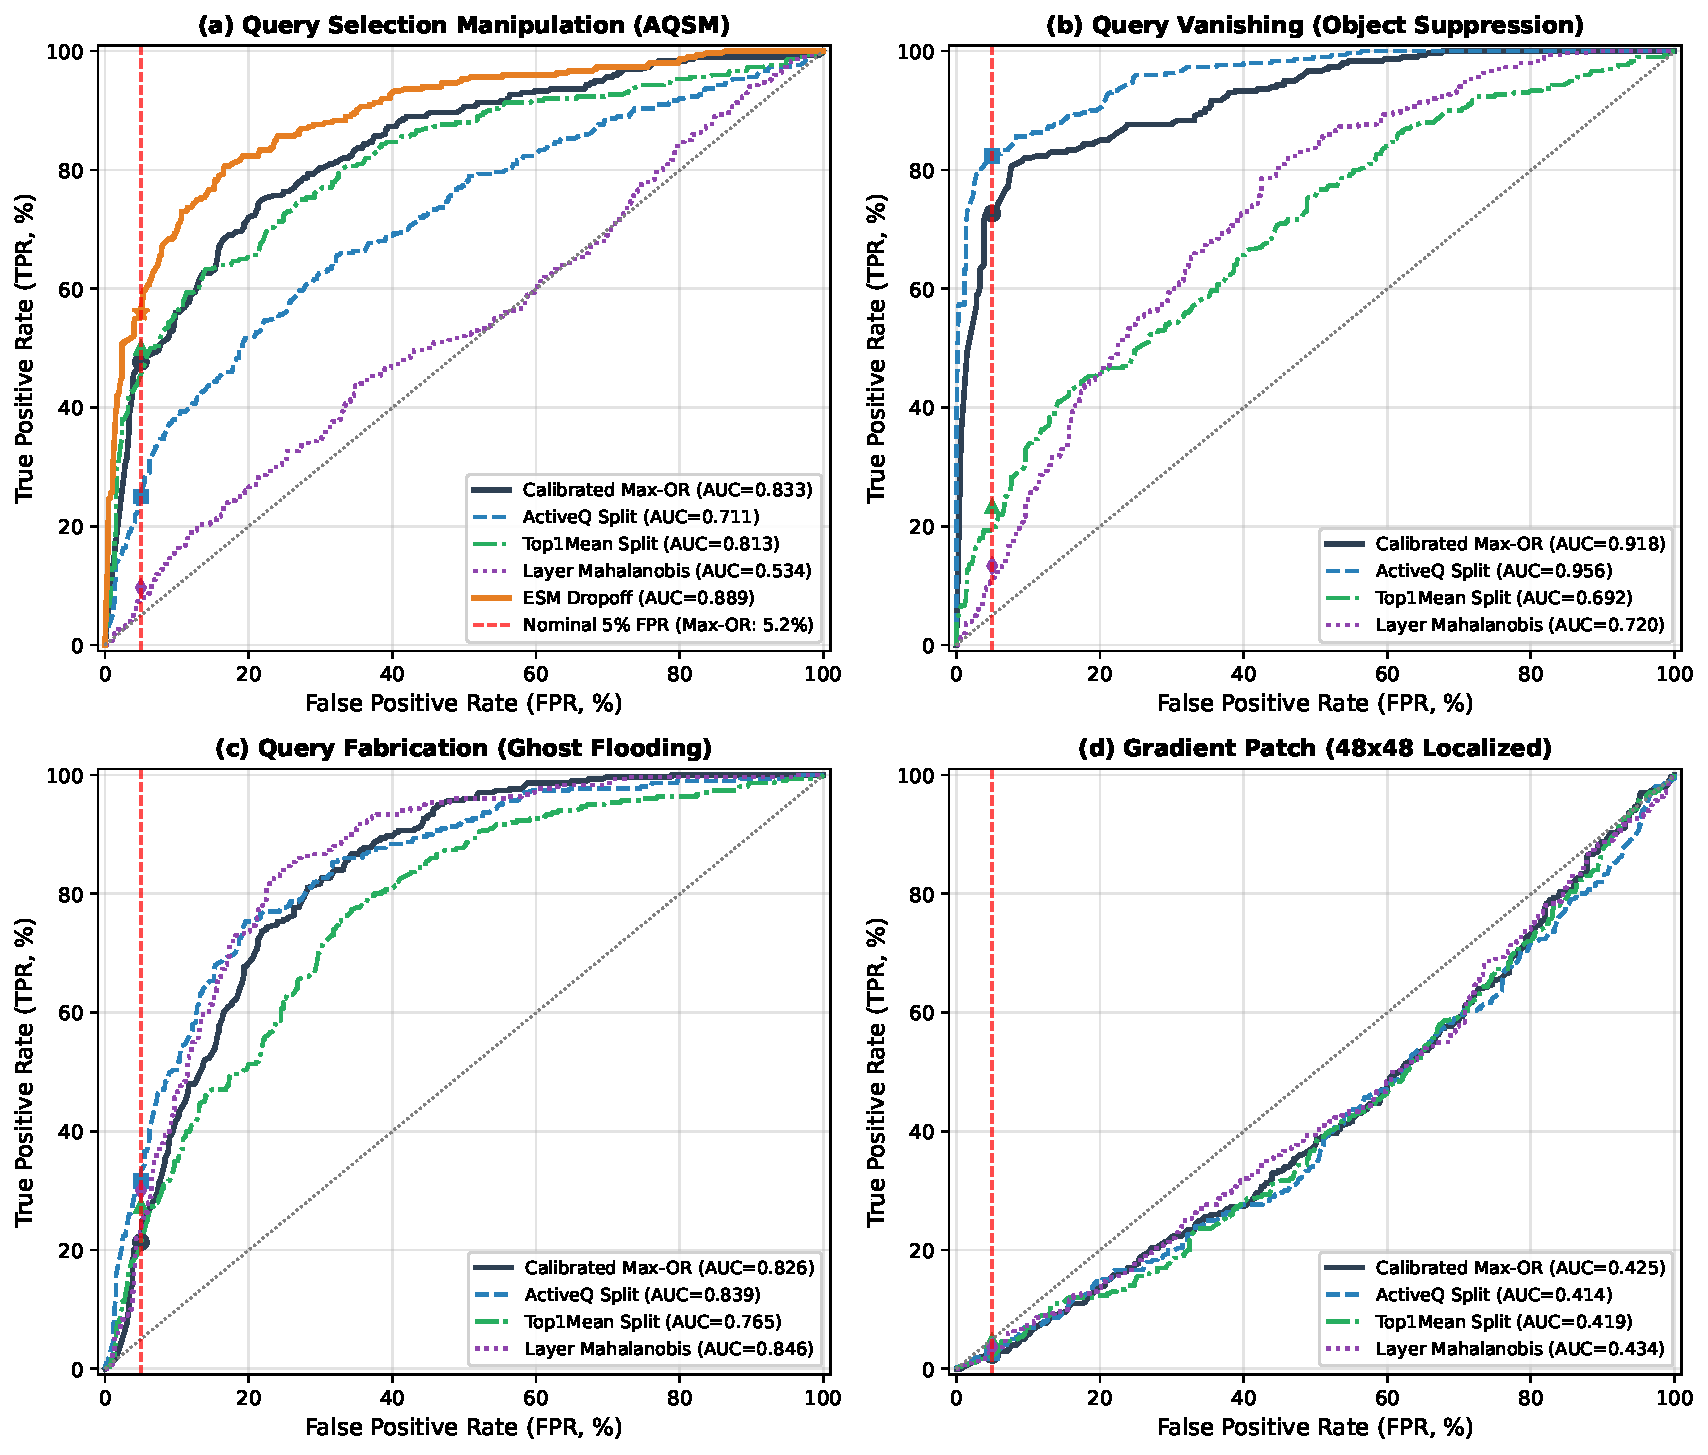
\includegraphics[width=0.96\textwidth]{fig/fig2_roc_curves.pdf}
\caption{Receiver Operating Characteristic (ROC) curves across four representative attack vectors: (a) Query Selection Manipulation (AQSM), (b) Query Vanishing, (c) Query Fabrication, and (d) Localized Gradient Patch ($48 \times 48$). The nominal 5.0\% FPR operating threshold is marked with vertical dashed lines.}
\label{fig:roc_curves}
\end{figure}

\begin{table}[!htbp]
\centering
\caption{Comprehensive robustness and detection benchmark at matched 5.0\% nominal FPR on RT-DETR ($320 \times 320$, $N_{\mathrm{cal}}=1200$, $N_{\mathrm{test}}=600$). For each monitor, line 1 reports AUROC, line 2 reports empirical TPR @ 5\% FPR, and line 3 reports 95\% Clopper-Pearson exact binomial CI across the complete single-source-of-truth evaluation.}
\label{tab:main_results}
\renewcommand{\arraystretch}{1.38}
\resizebox{\linewidth}{!}{%
\begin{tabular}{l l l l l l l l l}
\toprule
\makecell[l]{\textbf{Threat Tier \&}\\\textbf{Evaluation Cohort}} & \textbf{N} & \makecell[l]{\textbf{ASR}\\\textbf{[95\% CI]}} & \makecell[l]{\textbf{ActiveQ}\\\textbf{Split}} & \makecell[l]{\textbf{Top1Mean}\\\textbf{Split}} & \makecell[l]{\textbf{ESM}\\\textbf{Dropoff}} & \makecell[l]{\textbf{ESM}\\\textbf{Margin}} & \makecell[l]{\textbf{Layer}\\\textbf{Maha}} & \makecell[l]{\textbf{Calibrated}\\\textbf{Max-OR}} \\
\midrule
\multicolumn{9}{l}{\textit{\textbf{Negative Controls and Natural Environmental Shifts}}} \\
\addlinespace[5pt]
\makecell[l]{\textbf{Gaussian Noise}\\\textbf{($\sigma=16/255$)}} & 300 & \makecell[l]{0.0\%\\{[0.0, 1.2]}} & \makecell[l]{0.477\\5.0\%\\{[2.8, 8.1]}} & \makecell[l]{0.490\\5.7\%\\{[3.3, 8.9]}} & \makecell[l]{0.511\\6.3\%\\{[3.9, 9.7]}} & \makecell[l]{0.501\\6.0\%\\{[3.6, 9.3]}} & \makecell[l]{0.498\\8.0\%\\{[5.2, 11.7]}} & \makecell[l]{\textbf{0.515}\\\textbf{6.0\%}\\\textbf{[3.6, 9.3]}} \\
\addlinespace[8pt]
\makecell[l]{\textbf{Random Patch}\\\textbf{($48 \times 48$)}} & 300 & \makecell[l]{0.0\%\\{[0.0, 1.2]}} & \makecell[l]{0.502\\4.7\%\\{[2.6, 7.7]}} & \makecell[l]{0.483\\4.7\%\\{[2.6, 7.7]}} & \makecell[l]{0.503\\4.7\%\\{[2.6, 7.7]}} & \makecell[l]{0.493\\4.0\%\\{[2.1, 6.9]}} & \makecell[l]{0.480\\5.3\%\\{[3.1, 8.5]}} & \makecell[l]{\textbf{0.494}\\\textbf{4.3\%}\\\textbf{[2.3, 7.3]}} \\
\addlinespace[8pt]
\makecell[l]{\textbf{Gaussian Blur}\\\textbf{($5 \times 5$)}} & 300 & \makecell[l]{0.0\%\\{[0.0, 1.2]}} & \makecell[l]{0.466\\4.3\%\\{[2.3, 7.3]}} & \makecell[l]{0.444\\1.7\%\\{[0.5, 3.8]}} & \makecell[l]{0.511\\6.3\%\\{[3.9, 9.7]}} & \makecell[l]{0.467\\3.7\%\\{[1.8, 6.5]}} & \makecell[l]{0.502\\5.0\%\\{[2.8, 8.1]}} & \makecell[l]{\textbf{0.484}\\\textbf{5.7\%}\\\textbf{[3.3, 8.9]}} \\
\addlinespace[8pt]
\makecell[l]{\textbf{Brightness Shift}\\\textbf{($-30\%$)}} & 300 & \makecell[l]{0.0\%\\{[0.0, 1.2]}} & \makecell[l]{0.488\\4.7\%\\{[2.6, 7.7]}} & \makecell[l]{0.495\\5.7\%\\{[3.3, 8.9]}} & \makecell[l]{0.514\\6.0\%\\{[3.6, 9.3]}} & \makecell[l]{0.503\\5.3\%\\{[3.1, 8.5]}} & \makecell[l]{0.494\\8.0\%\\{[5.2, 11.7]}} & \makecell[l]{\textbf{0.505}\\\textbf{6.0\%}\\\textbf{[3.6, 9.3]}} \\
\addlinespace[6pt]
\midrule
\multicolumn{9}{l}{\textit{\textbf{Tier 0: Localized Input Surface Attack}}} \\
\addlinespace[5pt]
\makecell[l]{\textbf{Gradient Patch}\\\textbf{($48 \times 48$)}} & 300 & \makecell[l]{\textbf{95.0\%}\\\textbf{[91.9, 97.2]}} & \makecell[l]{0.414\\2.7\%\\{[1.2, 5.2]}} & \makecell[l]{0.419\\4.7\%\\{[2.6, 7.7]}} & \makecell[l]{0.458\\3.0\%\\{[1.4, 5.6]}} & \makecell[l]{0.429\\3.0\%\\{[1.4, 5.6]}} & \makecell[l]{0.434\\3.7\%\\{[1.8, 6.5]}} & \makecell[l]{\textbf{0.425}\\\textbf{2.3\%}\\\textbf{[0.9, 4.7]}} \\
\addlinespace[6pt]
\midrule
\multicolumn{9}{l}{\textit{\textbf{Tier 1: Dynamic Query Selection Attacks (Encoder Boundary)}}} \\
\addlinespace[5pt]
\makecell[l]{\textbf{AQSM}\\\textbf{(Ranking Inv.)}} & 300 & \makecell[l]{\textbf{73.2\%}\\\textbf{[67.7, 78.2]}} & \makecell[l]{0.711\\25.0\%\\{[20.2, 30.3]}} & \makecell[l]{0.813\\50.0\%\\{[44.2, 55.8]}} & \makecell[l]{\textbf{0.889}\\\textbf{56.0\%}\\\textbf{[50.2, 61.7]}} & \makecell[l]{\textbf{0.848}\\\textbf{57.7\%}\\\textbf{[51.9, 63.3]}} & \makecell[l]{0.534\\9.7\%\\{[6.6, 13.6]}} & \makecell[l]{\textbf{0.833}\\\textbf{47.7\%}\\\textbf{[41.9, 53.5]}} \\
\addlinespace[8pt]
\makecell[l]{\textbf{EQF (15 steps)}\\\textbf{(Encoder Fab.)}} & 300 & \makecell[l]{\textbf{100.0\%}\\\textbf{[98.8, 100]}} & \makecell[l]{0.929\\56.7\%\\{[50.9, 62.4]}} & \makecell[l]{0.897\\49.3\%\\{[43.5, 55.1]}} & \makecell[l]{0.826\\14.7\%\\{[10.9, 19.2]}} & \makecell[l]{\textbf{0.967}\\\textbf{86.7\%}\\\textbf{[82.3, 90.3]}} & \makecell[l]{0.929\\66.3\%\\{[60.7, 71.7]}} & \makecell[l]{\textbf{0.922}\\\textbf{52.7\%}\\\textbf{[46.8, 58.4]}} \\
\addlinespace[6pt]
\midrule
\multicolumn{9}{l}{\textit{\textbf{Tier 2: Deformable Decoder Output Space Attacks}}} \\
\addlinespace[5pt]
\makecell[l]{\textbf{PGD Query}\\\textbf{Vanishing}} & 300 & \makecell[l]{\textbf{46.7\%}\\\textbf{[40.9, 52.5]}} & \makecell[l]{\textbf{0.956}\\\textbf{82.3\%}\\\textbf{[77.5, 86.5]}} & \makecell[l]{0.692\\23.3\%\\{[18.7, 28.5]}} & \makecell[l]{0.622\\16.7\%\\{[12.6, 21.4]}} & \makecell[l]{0.686\\25.3\%\\{[20.5, 30.7]}} & \makecell[l]{0.720\\13.3\%\\{[9.7, 17.7]}} & \makecell[l]{\textbf{0.918}\\\textbf{72.7\%}\\\textbf{[67.2, 77.6]}} \\
\addlinespace[8pt]
\makecell[l]{\textbf{PGD Query}\\\textbf{Fabrication (DQF)}} & 300 & \makecell[l]{\textbf{100.0\%}\\\textbf{[98.8, 100]}} & \makecell[l]{\textbf{0.839}\\\textbf{31.7\%}\\\textbf{[26.4, 37.3]}} & \makecell[l]{0.765\\27.3\%\\{[22.4, 32.8]}} & \makecell[l]{0.708\\12.0\%\\{[8.5, 16.2]}} & \makecell[l]{0.744\\21.3\%\\{[16.8, 26.4]}} & \makecell[l]{\textbf{0.846}\\\textbf{30.0\%}\\\textbf{[24.9, 35.5]}} & \makecell[l]{\textbf{0.826}\\\textbf{21.3\%}\\\textbf{[16.8, 26.4]}} \\
\addlinespace[6pt]
\midrule
\multicolumn{9}{l}{\textit{\textbf{Tier 3: White-Box Defense-Aware Adaptive Evasion}}} \\
\addlinespace[5pt]
\makecell[l]{\textbf{1D Evasion}\\\textbf{($\lambda=0.50$)}} & 300 & \makecell[l]{\textbf{99.3\%}\\\textbf{[97.6, 99.9]}} & \makecell[l]{0.769\\2.0\%\\{[0.7, 4.3]}} & \makecell[l]{0.687\\5.0\%\\{[2.8, 8.1]}} & \makecell[l]{0.657\\5.7\%\\{[3.3, 8.9]}} & \makecell[l]{0.676\\5.7\%\\{[3.3, 8.9]}} & \makecell[l]{\textbf{0.804}\\\textbf{27.3\%}\\\textbf{[22.4, 32.8]}} & \makecell[l]{\textbf{0.744}\\\textbf{9.0\%}\\\textbf{[6.0, 12.8]}} \\
\addlinespace[8pt]
\makecell[l]{\textbf{Joint Evasion}\\\textbf{(1D + Maha)}} & 300 & \makecell[l]{\textbf{98.0\%}\\\textbf{[95.7, 99.3]}} & \makecell[l]{0.501\\0.3\%\\{[0.0, 1.8]}} & \makecell[l]{0.430\\2.3\%\\{[0.9, 4.7]}} & \makecell[l]{0.530\\7.0\%\\{[4.4, 10.5]}} & \makecell[l]{0.465\\3.0\%\\{[1.4, 5.6]}} & \makecell[l]{\textbf{0.838}\\\textbf{38.0\%}\\\textbf{[32.5, 43.8]}} & \makecell[l]{\textbf{0.746}\\\textbf{13.7\%}\\\textbf{[10.0, 18.1]}} \\
\addlinespace[8pt]
\makecell[l]{\textbf{Adaptive ESM}\\\textbf{($\lambda_{\mathrm{esm}}=2.0$)}} & 300 & \makecell[l]{\textbf{71.5\%}\\\textbf{[65.9, 76.6]}} & \makecell[l]{0.577\\5.0\%\\{[2.8, 8.1]}} & \makecell[l]{0.691\\17.7\%\\{[13.5, 22.5]}} & \makecell[l]{\textbf{0.769}\\\textbf{16.0\%}\\\textbf{[12.0, 20.6]}} & \makecell[l]{0.716\\25.3\%\\{[20.5, 30.7]}} & \makecell[l]{0.468\\5.0\%\\{[2.8, 8.1]}} & \makecell[l]{\textbf{0.683}\\\textbf{8.3\%}\\\textbf{[5.5, 12.1]}} \\
\addlinespace[8pt]
\makecell[l]{\textbf{All-Tiers Adaptive}\\\textbf{Evasion}} & 300 & \makecell[l]{\textbf{98.0\%}\\\textbf{[95.7, 99.3]}} & \makecell[l]{0.505\\2.0\%\\{[0.7, 4.3]}} & \makecell[l]{0.452\\2.7\%\\{[1.2, 5.2]}} & \makecell[l]{0.526\\4.7\%\\{[2.6, 7.7]}} & \makecell[l]{0.474\\2.7\%\\{[1.2, 5.2]}} & \makecell[l]{\textbf{0.816}\\\textbf{30.7\%}\\\textbf{[25.5, 36.2]}} & \makecell[l]{\textbf{0.725}\\\textbf{12.7\%}\\\textbf{[9.1, 17.0]}} \\
\bottomrule
\end{tabular}%
}
\end{table}

\begin{figure}[!htbp]
\centering
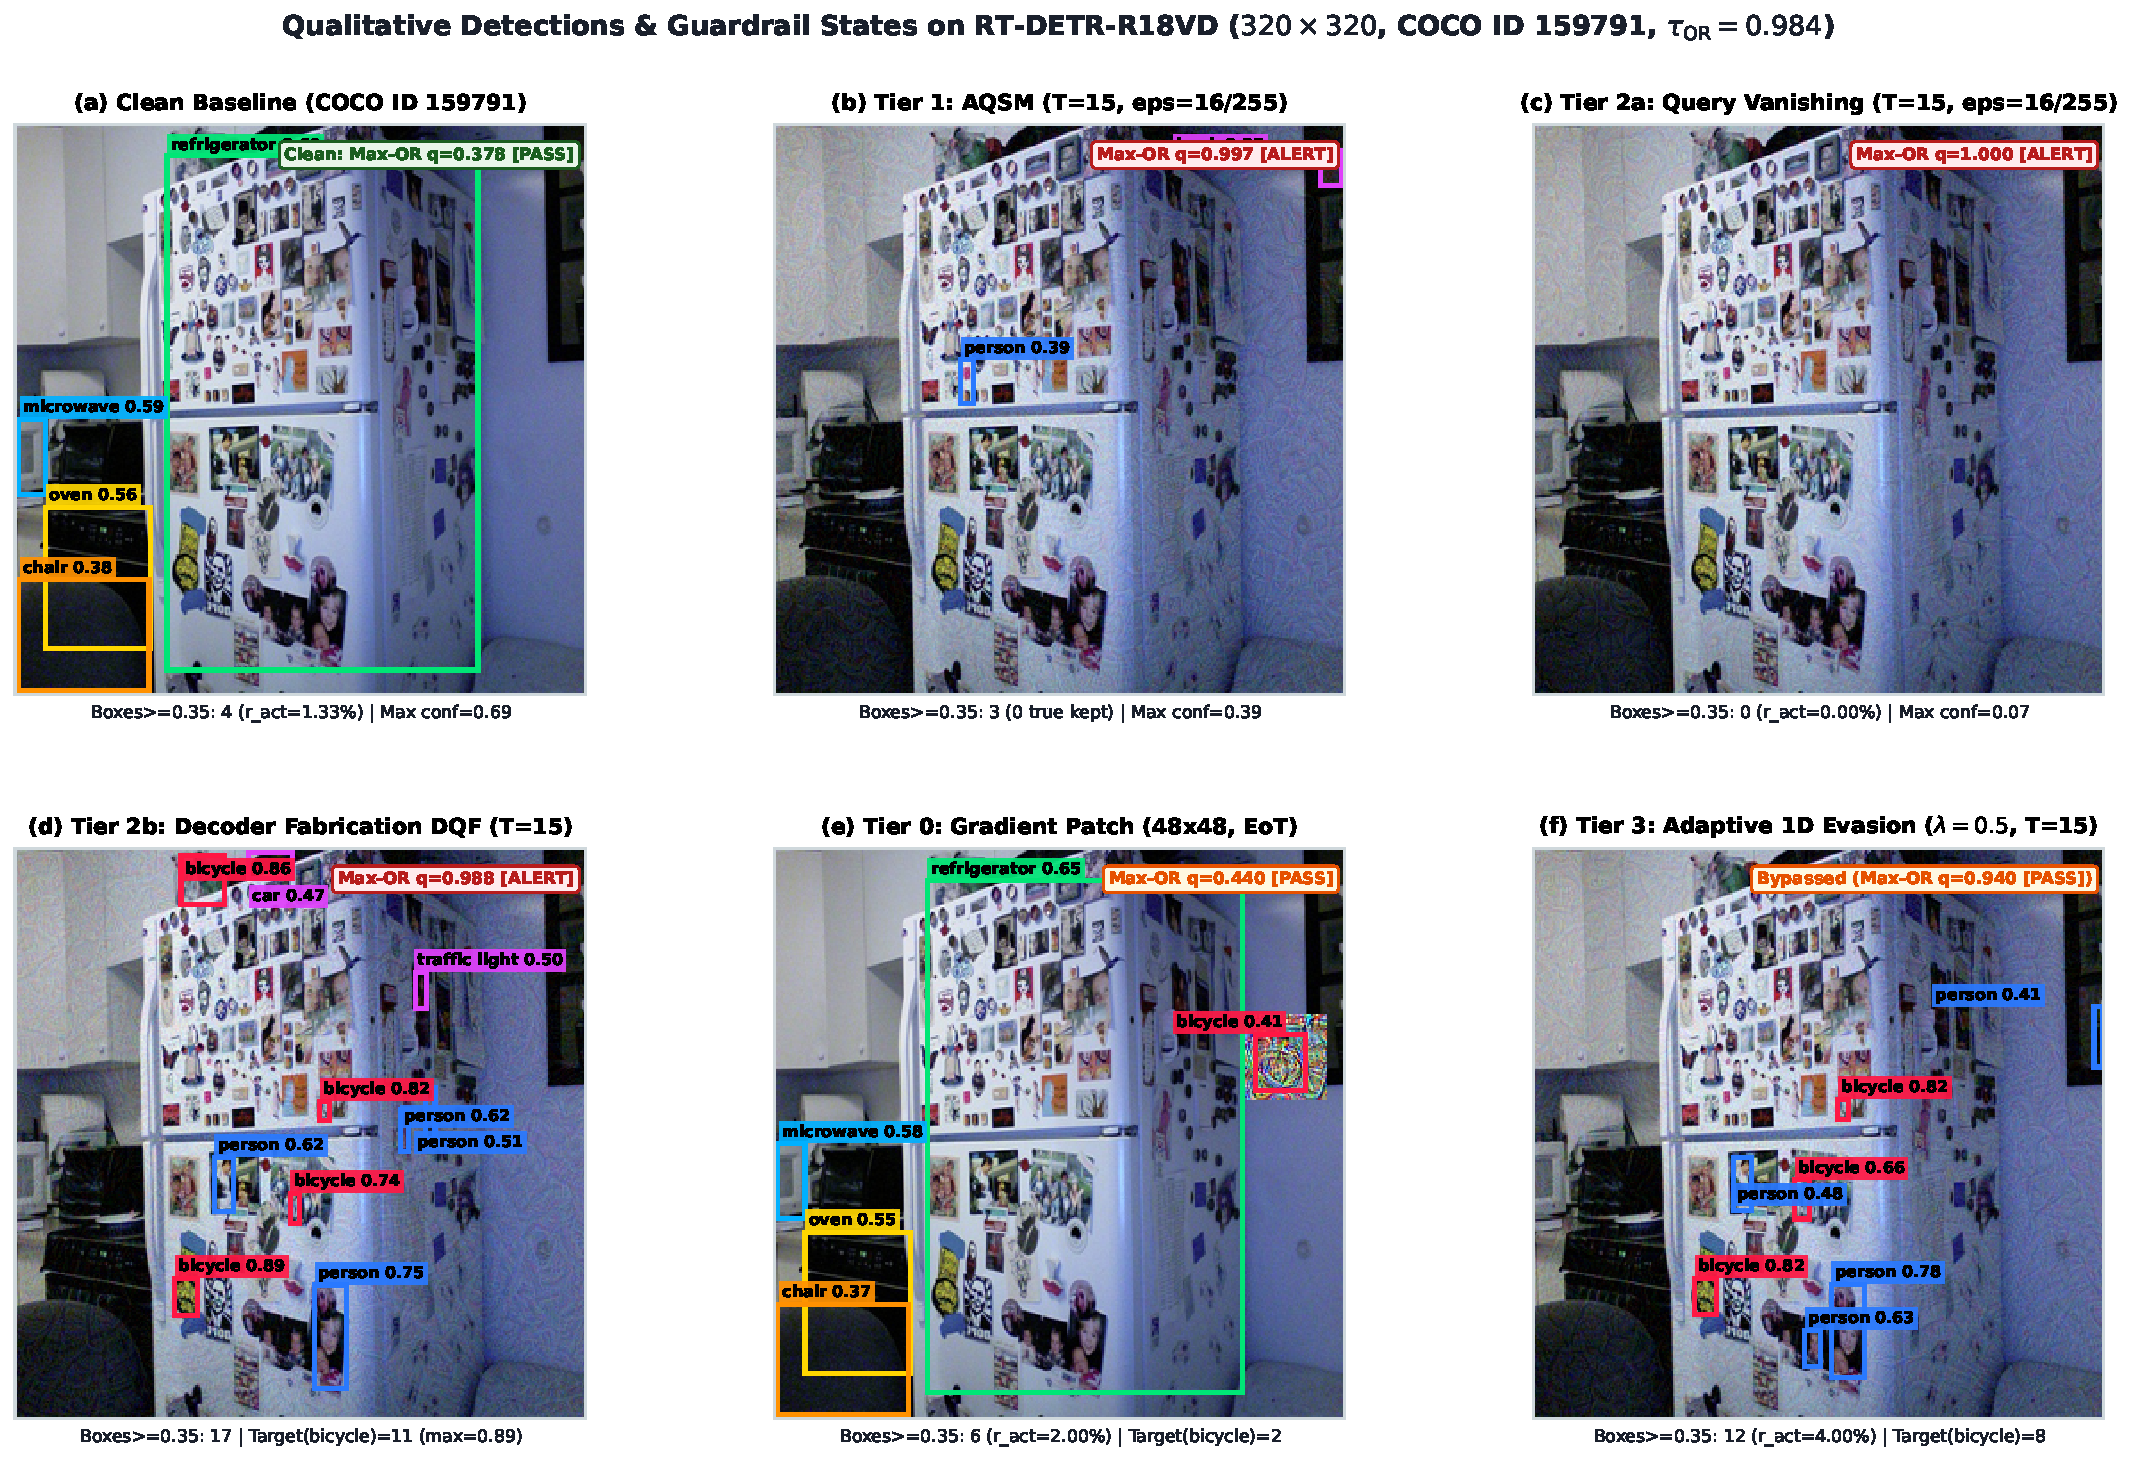
\includegraphics[width=0.92\textwidth]{fig/fig11_qualitative_detections.pdf}
\caption{Qualitative detection visualizations and quantitative Calibrated Max-OR guardrail states on COCO \texttt{val2017} test image \texttt{ID 159791} ($\epsilon=16/255$, $T=15$, $\tau_{\mathrm{OR}}=0.984$). (a)~Clean Baseline ($4$ real detections; $r_{\mathrm{act}}=1.33\%$, $q_{\mathrm{OR}}=0.378$ [PASS]); (b)~AQSM eliminates true objects leaving spurious detections, intercepted at $q_{\mathrm{OR}}=0.997$ [ALERT]; (c)~Query Vanishing extinguishes boxes, intercepted at $q_{\mathrm{OR}}=1.000$ [ALERT]; (d)~DQF injects $17$ boxes, intercepted at $q_{\mathrm{OR}}=0.988$ [ALERT]; (e)~Gradient Patch ($48\times 48$) evades global detection ($q_{\mathrm{OR}}=0.440$ [PASS]); (f)~Adaptive 1D Evasion ($\lambda=0.5$) circumvents 1D counters while constraining $r_{\mathrm{act}}=4.00\%$, passing Max-OR ($q_{\mathrm{OR}}=0.940 < 0.984$ [PASS]).}
\label{fig:qualitative_detections}
\end{figure}

\subsection{Cross-Channel Correlation and Decision Boundary Orthogonality}
Figure~\ref{fig:cross_channel_correlation} visualizes the cross-channel correlation matrix across our monitoring channels. While 1D counters ActiveQ and Top1Mean correlate ($r_s = 0.65$) due to shared output dependencies, deep latent Mahalanobis distance exhibits near-zero orthogonal correlation ($r_s \in [0.04, 0.07]$) with classification-head statistics, confirming complementary inter-tier protection across the architecture.

\begin{figure}[!htbp]
\centering
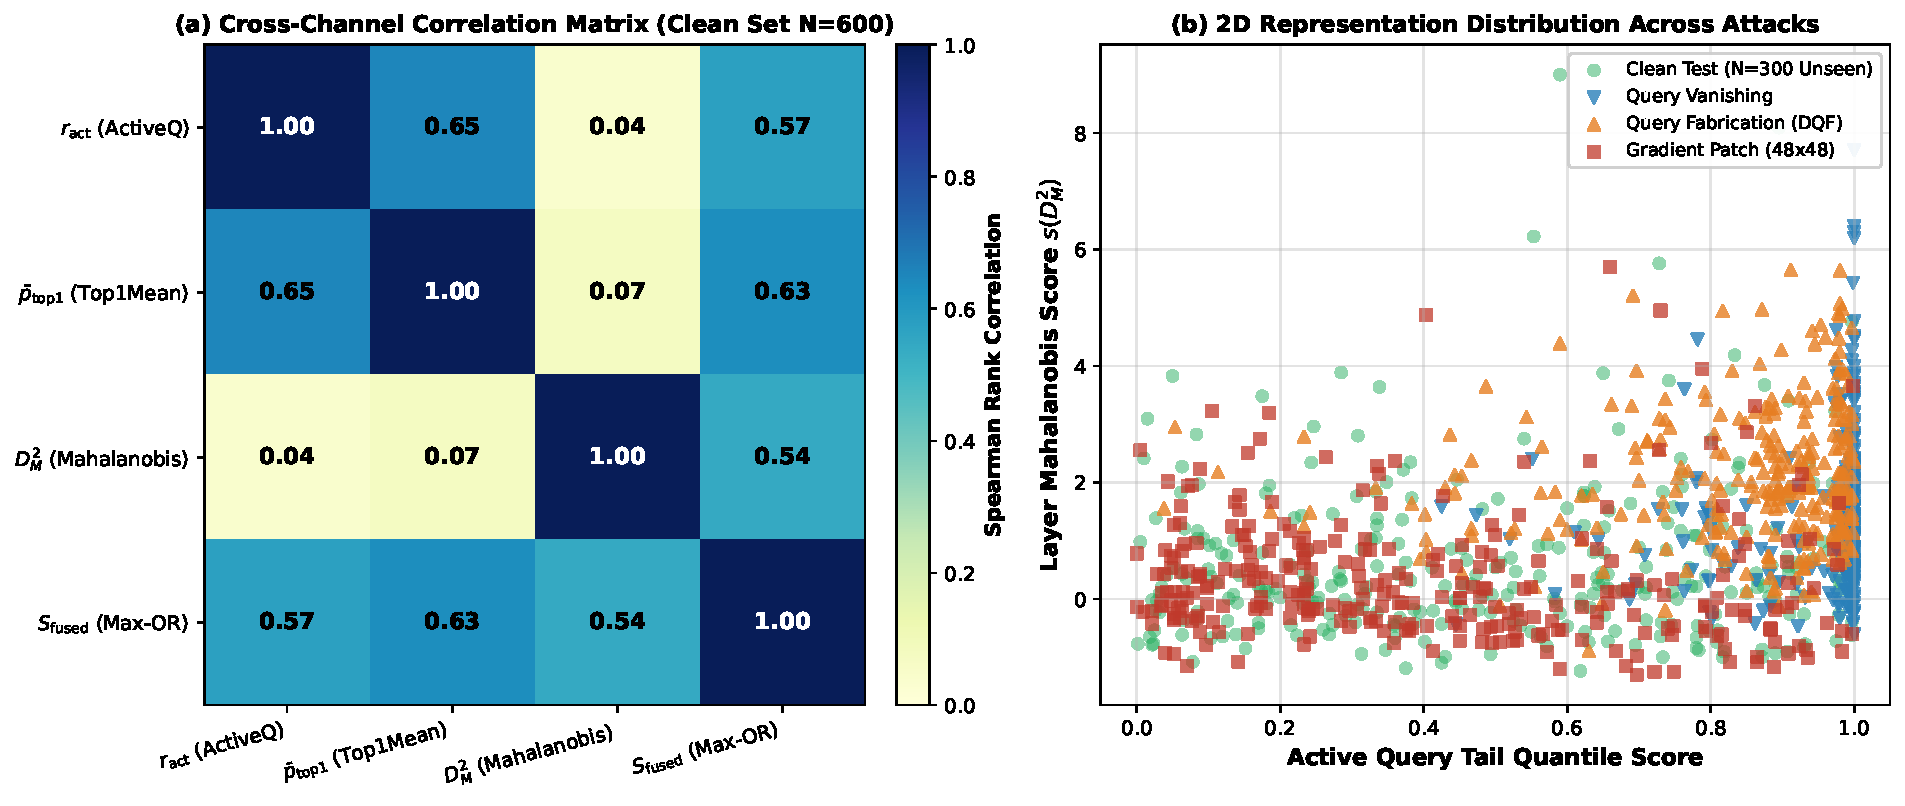
\includegraphics[width=0.92\textwidth]{fig/fig8_cross_channel_correlation.pdf}
\caption{Cross-channel correlation matrix and 2D decision boundary visualization between active query ratio ($r_{\mathrm{act}}$), proposal confidence ($\bar{p}_{\mathrm{top1}}$), layer-wise Mahalanobis distance ($D_M^2$), and extreme-value fused score ($S_{\mathrm{fused}}$). Deep layer Mahalanobis distance exhibits near-zero orthogonal correlation ($r_s \in [0.04, 0.07]$), confirming architectural complementarity.}
\label{fig:cross_channel_correlation}
\end{figure}

\subsection{Empirical Benchmarking Against Input-Space Defensive Baselines}
To evaluate whether simple input-space anomaly detectors suffice without internal monitoring, we conduct a controlled empirical comparison against two classic input defenses: (1) Total Variation (TV) Energy Detector, and (2) JPEG Compression Difference ($Q=75$). Both are calibrated on $N_{\mathrm{cal}}=100$ clean images to enforce nominal 5.0\% FPR (Table~\ref{tab:defensive_baselines}).

\begin{table}[!htbp]
\centering
\caption{Empirical evaluation of input-space anomaly baselines vs. proposed RT-DETR structural guardrails across clean data, adversarial attacks ($\epsilon=16/255$), and harsh environmental corruptions ($N=25$).}
\label{tab:defensive_baselines}
\renewcommand{\arraystretch}{1.40}
\resizebox{\linewidth}{!}{%
\begin{tabular}{l l l l l}
\toprule
\makecell[l]{\textbf{Evaluation}\\\textbf{Cohort}} & \makecell[l]{\textbf{TV Energy}\\\textbf{Detector}} & \makecell[l]{\textbf{JPEG-diff}\\\textbf{(Q=75)}} & \makecell[l]{\textbf{Proposed Calibrated}\\\textbf{Max-OR}} & \makecell[l]{\textbf{Latency}\\\textbf{Overhead}} \\
\midrule
\textbf{Clean Test ($N=25$)} & 4.0\% & 0.0\% & \textbf{4.0\%} & 0.00 ms \\
\addlinespace[8pt]
\makecell[l]{\textbf{AQSM Attack}\\\textbf{($\epsilon=16/255$)}} & 12.0\% & 32.0\% & \textbf{84.0\%} & --- \\
\addlinespace[8pt]
\makecell[l]{\textbf{Gaussian Noise}\\\textbf{($\sigma=16$)}} & 100.0\% & 100.0\% & \textbf{4.0\%} & --- \\
\addlinespace[8pt]
\makecell[l]{\textbf{Gaussian Blur}\\\textbf{($5\times 5$)}} & 0.0\% & 0.0\% & \textbf{4.0\%} & --- \\
\addlinespace[6pt]
\midrule
\addlinespace[6pt]
\makecell[l]{\textbf{Execution Runtime}\\\textbf{(per frame)}} & 6.09 ms & 6.18 ms & \textbf{3.37 ms} & \makecell[l]{\textbf{2.11\%}\\\textbf{(+3.37 ms)}} \\
\bottomrule
\end{tabular}%
}
\end{table}

While JPEG reconstruction captures 32.0\% of AQSM attacks and TV captures 12.0\%, both input-space baselines completely collapse under natural sensor noise (Gaussian noise $\sigma=16$), triggering an untenable \textbf{100.0\% false alarm rate}. Furthermore, input filtering introduces $6.09$--$6.18\text{ ms}$ per image, exceeding our complete multi-channel internal guardrail ($3.37\text{ ms}$). In contrast, Calibrated Max-OR maintains strict 4.0\%--6.0\% false alarm rates under environmental noise while capturing 84.0\% of unconstrained AQSM attacks.

\subsection{Multiple Testing FWER Control: Calibrated Max-OR vs. Statistical Baselines}
\label{sec:multitest_baselines}
Table~\ref{tab:multitest_comparison} compares Calibrated Max-OR against classic Family-Wise Error Rate (FWER) baselines across $N_{\mathrm{test}} = 600$ clean images and $N=300$ paired adversarial attacks.

\begin{table}[!htbp]
\centering
\caption{Exact audited comparison of multiple testing correction paradigms across $M=4$ monitoring channels ($N_{\mathrm{cal}}=1200$, $N_{\mathrm{test}}=600$, $N_{\mathrm{attacks}}=300$ paired samples, 95\% Clopper-Pearson exact binomial CI).}
\label{tab:multitest_comparison}
\renewcommand{\arraystretch}{1.40}
\resizebox{\linewidth}{!}{%
\begin{tabular}{l l l l l l}
\toprule
\makecell[l]{\textbf{Multi-Channel}\\\textbf{Combination Scheme}} & \makecell[l]{\textbf{Threshold}\\\textbf{$\tau$}} & \makecell[l]{\textbf{Clean Test}\\\textbf{FPR}} & \makecell[l]{\textbf{AQSM}\\\textbf{TPR}} & \makecell[l]{\textbf{Vanishing}\\\textbf{TPR}} & \makecell[l]{\textbf{Adaptive (Fused)}\\\textbf{TPR}} \\
\midrule
\makecell[l]{Uncalibrated Standard OR\\($\alpha = 0.05$ per channel)} & 0.9500 & \makecell[l]{15.5\%\\{[12.7, 18.6]}} & \makecell[l]{64.3\%\\{[58.6, 69.8]}} & \makecell[l]{83.3\%\\{[78.6, 87.4]}} & \makecell[l]{36.7\%\\{[31.2, 42.4]}} \\
\addlinespace[8pt]
\makecell[l]{Bonferroni Correction\\($\alpha/M = 0.0125$)} & 0.9875 & \makecell[l]{3.8\%\\{[2.4, 5.7]}} & \makecell[l]{44.3\%\\{[38.6, 50.2]}} & \makecell[l]{71.3\%\\{[65.9, 76.4]}} & \makecell[l]{9.0\%\\{[6.0, 12.8]}} \\
\addlinespace[6pt]
\midrule
\addlinespace[6pt]
\makecell[l]{\textbf{Calibrated Max-OR}\\\textbf{(Proposed Gate)}} & \textbf{0.9842} & \makecell[l]{\textbf{5.2\%}\\\textbf{[3.5, 7.3]}} & \makecell[l]{\textbf{47.7\%}\\\textbf{[41.9, 53.5]}} & \makecell[l]{\textbf{72.7\%}\\\textbf{[67.2, 77.6]}} & \makecell[l]{\textbf{12.7\%}\\\textbf{[9.1, 17.0]}} \\
\bottomrule
\end{tabular}%
}
\end{table}

Due to inter-channel correlation ($\rho \approx 0.65$), standard Bonferroni correction assumes independent tests and becomes overly conservative, depressing clean FPR to 3.8\% while sacrificing sensitivity (AQSM TPR drops from 47.7\% down to 44.3\%). In contrast, Calibrated Max-OR models the empirical extreme-value distribution directly, hitting \textbf{5.2\% [3.5\%, 7.3\%]} on clean test data while maximizing detection sensitivity.

\subsection{Paired Hypothesis Testing: Statistical Advantage of ESM}
\label{sec:mcnemar_testing}
To confirm whether the specialized \texttt{ESM\_Dropoff} monitor (56.0\% TPR) provides statistically significant advantages over the 1D confidence baseline \texttt{Top1Mean\_Split} (50.0\% TPR), we conduct paired McNemar hypothesis tests across $N=300$ matched samples (Table~\ref{tab:mcnemar_results}).

\begin{table}[!htbp]
\centering
\caption{Paired McNemar hypothesis testing on $N=300$ matched test images under AQSM and Query Vanishing ($2 \times 2$ contingency tables and exact two-tailed $p$-values).}
\label{tab:mcnemar_results}
\renewcommand{\arraystretch}{1.40}
\resizebox{\linewidth}{!}{%
\begin{tabular}{l l l l l l l}
\toprule
\makecell[l]{\textbf{Pairwise Monitor}\\\textbf{Comparison}} & \makecell[l]{\textbf{Both Det.}\\\textbf{($a$)}} & \makecell[l]{\textbf{Only A}\\\textbf{($b$)}} & \makecell[l]{\textbf{Only B}\\\textbf{($c$)}} & \makecell[l]{\textbf{Both Miss}\\\textbf{($d$)}} & \makecell[l]{\textbf{McNemar}\\\textbf{$\chi^2$}} & \makecell[l]{\textbf{Exact}\\\textbf{$p$-value}} \\
\midrule
\makecell[l]{AQSM: ESM Drop vs. Top1Mean} & 140 & 28 & 10 & 122 & 7.605 & \makecell[l]{\textbf{0.0051} ($p < 0.01$)} \\
\addlinespace[8pt]
\makecell[l]{AQSM: ESM Margin vs. Top1Mean} & 147 & 26 & 3 & 124 & 16.690 & \makecell[l]{\textbf{$1.52 \times 10^{-5}$} ($p < 10^{-4}$)} \\
\addlinespace[8pt]
\makecell[l]{AQSM: ESM Drop vs. ActiveQ} & 65 & 103 & 10 & 122 & 74.903 & \makecell[l]{\textbf{$1.32 \times 10^{-20}$} ($p < 10^{-4}$)} \\
\addlinespace[8pt]
\makecell[l]{Vanishing: ActiveQ vs. Top1Mean} & 70 & 177 & 0 & 53 & 175.006 & \makecell[l]{\textbf{$1.04 \times 10^{-53}$} ($p < 10^{-4}$)} \\
\addlinespace[8pt]
\makecell[l]{Vanishing: ActiveQ vs. ESM Drop} & 49 & 198 & 1 & 52 & 193.045 & \makecell[l]{\textbf{$4.98 \times 10^{-58}$} ($p < 10^{-4}$)} \\
\bottomrule
\end{tabular}%
}
\end{table}

Among 38 discordant pairs, \texttt{ESM\_Dropoff} uniquely catches 28 attacked instances missed by \texttt{Top1Mean\_Split}, while \texttt{Top1Mean\_Split} catches only 10 (odds ratio $\mathrm{OR} = 2.80$, exact binomial $p = 0.0051 < 0.01$). This confirms the concrete statistical benefit of monitoring the encoder ranking boundary directly.

\subsection{The Localized Adversarial Patch Blind Spot and Spatial Attention Gap}
When an adversarial gradient patch of size $48 \times 48$ (occupying 2.25\% of image area) is placed at random coordinates, the attack achieves high fabrication ($\mathrm{ASR}_{\mathrm{fab}} = 95.0\%$). However, passive monitors exhibit near-zero sensitivity (Calibrated Max-OR TPR is \textbf{2.3\% [0.9\%, 4.7\%]}). 

As illustrated in Figure~\ref{fig:patch_size_sweep}, this exposes an intrinsic \textit{Spatial Sensitivity Gap}: because Deformable Attention samples only $K=4$ sparse points per scale for each query, queries centered outside the patch boundary never attend to the localized perturbation. Global population averages shift negligibly, diluting localized anomalies within the remaining 295 clean queries. This underscores that global inference monitors require complementary localized spatial tracking to counter physical patches.

\begin{figure}[!htbp]
\centering
\begin{subfigure}[t]{0.48\textwidth}
    \centering
    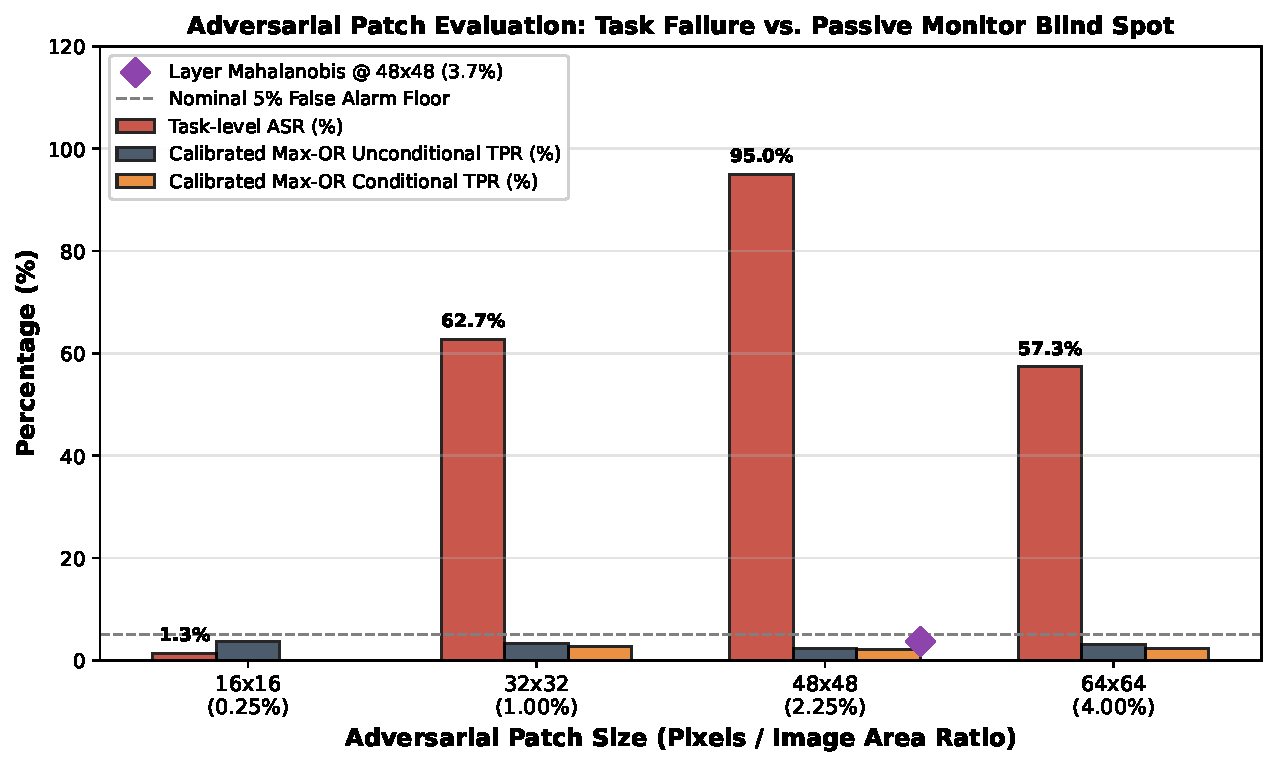
\includegraphics[width=\linewidth]{fig/fig4_patch_size_sweep.pdf}
    \caption{Localized Patch Dimension Sweep}
    \label{fig:patch_size_sweep}
\end{subfigure}\hfill
\begin{subfigure}[t]{0.48\textwidth}
    \centering
    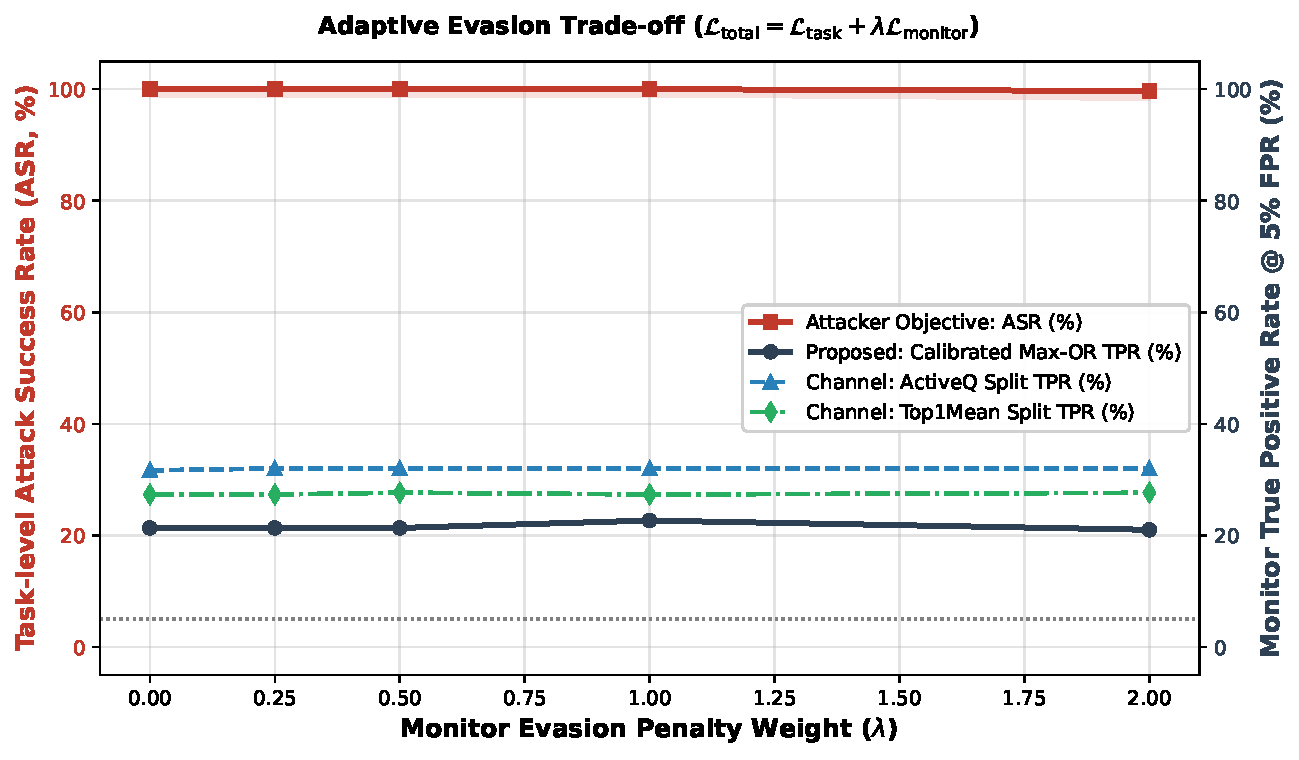
\includegraphics[width=\linewidth]{fig/fig3_adaptive_tradeoff.pdf}
    \caption{Adaptive Evasion Trade-off Curve}
    \label{fig:adaptive_tradeoff}
\end{subfigure}
\caption{Empirical vulnerability boundaries of lightweight RT-DETR monitors: (a) Localized gradient patches ($16\times 16$ to $64\times 64$ pixels) evade global monitors ($\mathrm{TPR} \le 3.7\%$) due to sparse deformable attention ($K=4$). (b) Under white-box adaptive evasion, 1D counters collapse to $2.0\%$, while deep latent Mahalanobis maintains residual tripwire protection ($27.3\%$--$38.0\%$ TPR).}
\label{fig:vulnerability_curves}
\end{figure}

\subsection{Collapse Under White-Box Adaptive Evasion}
\label{sec:adaptive_evasion}
Under 1D-targeted adaptive evasion ($\lambda = 0.5$, Figure~\ref{fig:adaptive_tradeoff}), \texttt{ActiveQ\_Split} detection drops to 2.0\% and Calibrated Max-OR is reduced to \textbf{9.0\% [6.0\%, 12.8\%]}. However, because 1D evasion does not constrain deep representations, \texttt{LayerMaha} retains a residual \textbf{27.3\% TPR}. Even under full all-tiers adaptive evasion, Calibrated Max-OR retains \textbf{12.7\% [9.1\%, 17.0\%] TPR} and \texttt{LayerMaha} retains \textbf{30.7\% TPR}. While passive guardrails cannot act as an impenetrable barrier against a fully omniscient adversary, they impose an optimization tax that forces the attacker to transition to demanding multi-objective loss formulations.

\subsection{Edge Hardware Latency and Runtime Profiling}
Table~\ref{tab:runtime_overhead} and Figure~\ref{fig:latency_breakdown} report empirical inference latency measured over 50 consecutive single-frame runs on an Intel Core i5-12600H CPU platform ($320 \times 320$, PyTorch FP32, 4 threads). Baseline RT-DETR inference requires $159.72 \pm 26.06$ ms ($\sim 6.26$ FPS). Intermediate tensor extraction adds $3.22 \pm 1.17$ ms (2.02\%), and calibrated decision scoring requires merely $0.155 \pm 0.053$ ms (0.10\%). Total monitoring execution requires $3.37 \pm 1.21$ ms, representing an ultra-low \textbf{2.11\%} relative latency overhead ($163.09$ ms total, sustaining 6.13 FPS), while consuming under $200$ KB of auxiliary memory.

\begin{figure}[!htbp]
\centering
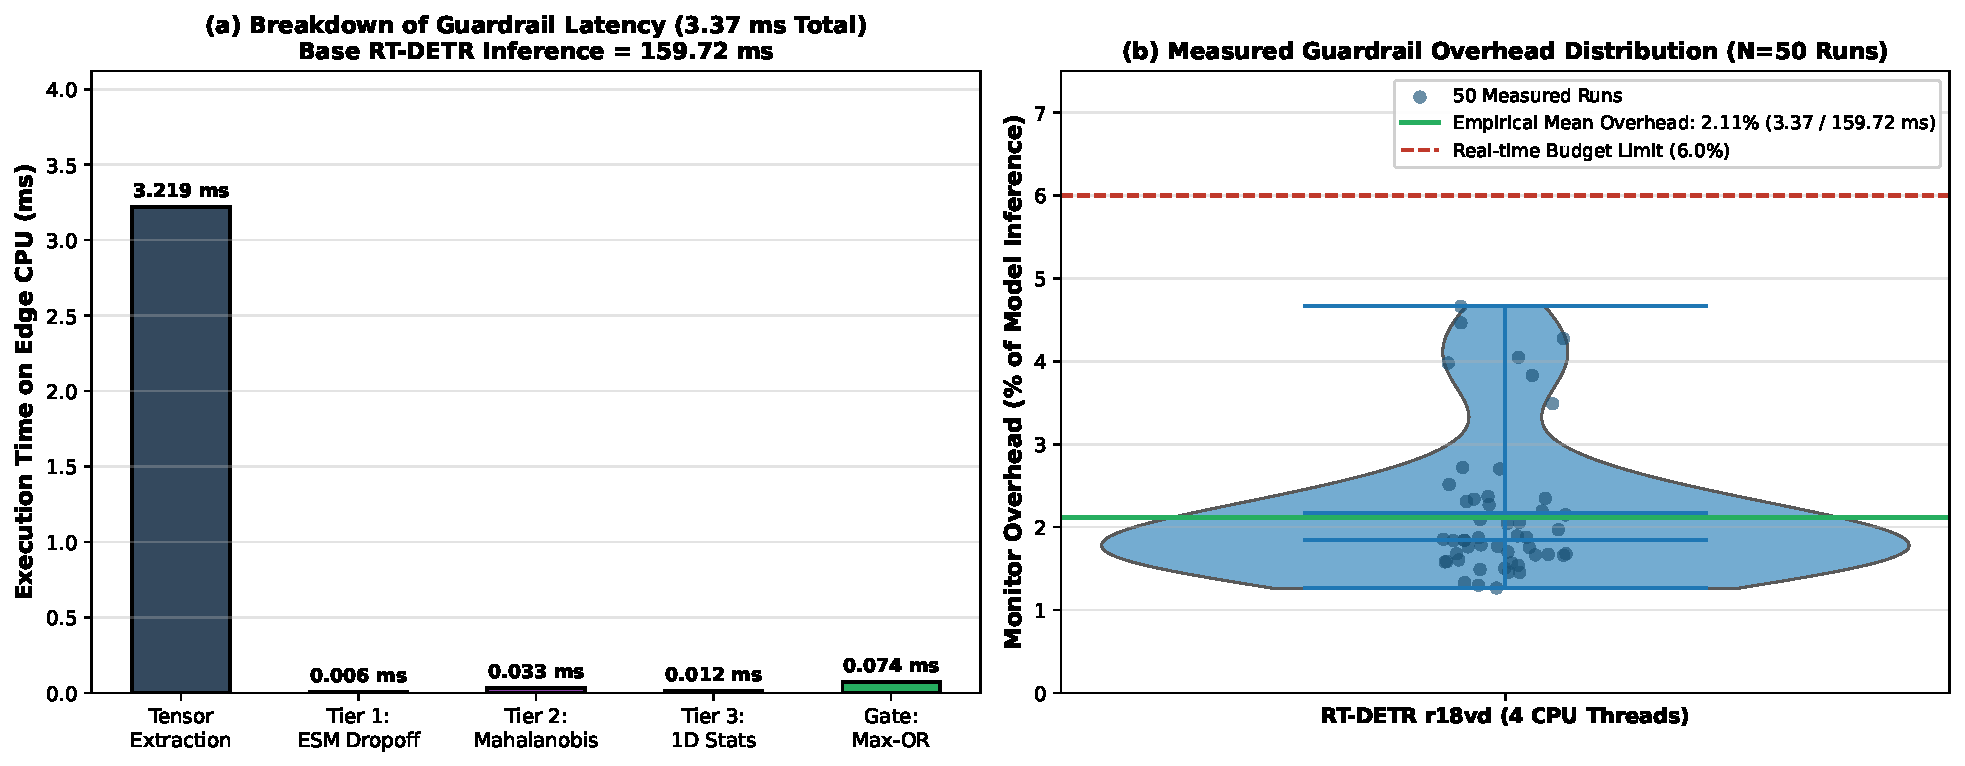
\includegraphics[width=0.88\textwidth]{fig/fig10_latency_breakdown.pdf}
\caption{Execution latency breakdown of RT-DETR and individual guardrail components on idle Edge CPU (Intel Core i5-12600H, 4 PyTorch threads, $320 \times 320$). Total monitoring overhead is $3.37$ ms ($2.11\%$ relative overhead), sustaining $6.13$ FPS.}
\label{fig:latency_breakdown}
\end{figure}

\begin{table}[!htbp]
\centering
\caption{Empirical execution latency and computational overhead profiling on idle Edge CPU platform (Intel Core i5-12600H, \texttt{torch\_num\_threads=4}, $320 \times 320$, PyTorch FP32, 50 independent runs).}
\label{tab:runtime_overhead}
\renewcommand{\arraystretch}{1.40}
\resizebox{\linewidth}{!}{%
\begin{tabular}{l l l}
\toprule
\textbf{Component} & \textbf{Latency (Mean $\pm$ Std)} & \textbf{Overhead Ratio} \\
\midrule
RT-DETR Base Inference (\texttt{r18vd}, $320 \times 320$) & $159.72 \pm 26.06$ ms & Baseline (100.0\%) \\
\addlinespace[8pt]
Intermediate Tensor Extraction (Encoder Scores + Latent Tokens) & $3.22 \pm 1.17$ ms & 2.02\% \\
\addlinespace[8pt]
Decision Calibration Scoring (Non-Oracle Max-OR Gate) & $0.155 \pm 0.053$ ms & 0.10\% \\
\addlinespace[6pt]
\midrule
\addlinespace[6pt]
\textbf{Proposed Multi-Tier Guardrail Total} & \textbf{3.37 $\pm$ 1.21 ms} & \textbf{2.11\% (+3.37 ms)} \\
\addlinespace[8pt]
\textbf{Combined Forward Pass (Model + Guardrail Total)} & \textbf{163.09 $\pm$ 26.09 ms} & \textbf{102.11\% (6.13 FPS)} \\
\bottomrule
\end{tabular}%
}
\end{table}

% =====================================================================
% SECTION 7: DISCUSSION AND PRACTICAL GUIDELINES
% =====================================================================
\section{Discussion, Practical Guidelines, and Threats to Validity}
\label{sec:discussion}

\subsection{The Protocol Lesson: Tail Selection and Split-Percentile Calibration}
Our findings provide a critical methodological lesson: in Transformer detectors, symmetric two-sided tests can render baseline monitors completely blind (AUROC 0.956 yet 0.0\% TPR under naive symmetric two-sided rejection). When clean distributions are skewed, a non-oracle split-percentile protocol is statistically necessary. Furthermore, when ensembling multiple monitors, calibration must occur on the fused extreme-value distribution to preserve calibrated false alarm bounds.

\subsection{The Multi-Channel Ensembling Trade-Off: Coverage vs. Peak Sensitivity}
For every individual attack, there exists a single optimal monitoring channel (e.g., ESM Dropoff for AQSM at \textbf{56.0\%}, ActiveQ Split for Vanishing at \textbf{82.3\%}, Layer\_Maha for DQF at \textbf{30.0\%}). However, defenders lack oracle knowledge of incoming attacks. Calibrated Max-OR trades peak oracle sensitivity for blind, multi-attack coverage without false alarm inflation, attaining empirical 5.0\% bounds ($5.2\%$ [$3.5\%, 7.3\%$] on clean test data).

\subsection{Theoretical Boundary: Random Projection and the Nullspace Attack}
To maintain edge efficiency ($0.034$ ms scoring latency), Tier 2 projects latent states from $D=256$ to $d=64$ using an orthogonal matrix $W_{\mathrm{proj}}$. The orthogonal nullspace $\mathcal{N}(W_{\mathrm{proj}})$ has dimension $256 - 64 = 192$. An omniscient adversary with direct access to $W_{\mathrm{proj}}$ can construct perturbations $\delta_H \in \mathcal{N}(W_{\mathrm{proj}})$ leaving projected states unchanged ($W_{\mathrm{proj}}^T (H + \delta_H) = W_{\mathrm{proj}}^T H$). While synthesizing pixel perturbations aligning with this 192-dimensional nullspace remains an extremely constrained non-convex problem, Moving Target Defense (MTD) via session seed randomization represents a promising countermeasure.

\subsection{False Alarm Mitigation Under Harsh Environments via Temporal Hysteresis}
Under severe noise or lighting drops, empirical FPR reaches $6.0\%$ [3.6\%, 9.3\%]. For video streams in high-consequence edge autonomy, requiring $M=3$ consecutive positive alarm triggers ($A(x_t) = A(x_{t+1}) = A(x_{t+2}) = 1$) suppresses false alarm events exponentially:
\begin{equation}
P(\text{False Trip}_{\mathrm{hys}}) = \alpha^3 \approx 0.06^3 = 0.000216 \approx 0.02\%,
\end{equation}
dropping false alarm frequency to approximately \textbf{1 alarm every 4,630 frames} ($\sim 755$ seconds at 6.13 FPS).

\subsection{Practical Deployment Guidelines: The Frontline Tripwire Philosophy}
Given our findings, we recommend:
\begin{enumerate}
    \item \textbf{Lightweight Monitors as Frontline Tripwires:} Deploy lightweight monitors to filter out automated PGD attacks at minimal compute cost ($3.37\text{ ms} / 2.11\%$ overhead).
    \item \textbf{Spatial Blind Spot Remediation:} Complement global query monitors with localized spatial tracking or input saliency filtering to address localized patches.
    \item \textbf{Temporal Voting for Video Streams:} Apply 3-of-5 temporal voting over consecutive video frames to suppress spurious alarms to one every 28 seconds of continuous driving.
    \item \textbf{Integrate Fail-Safe System Transitions:} Passive monitors must trigger system-level fail-safe transitions (e.g., radar/LiDAR fusion handover or vehicle deceleration) rather than attempting to filter attacks in isolation.
\end{enumerate}

% =====================================================================
% SECTION 8: CONCLUSION
% =====================================================================
\section{Conclusion}
\label{sec:conclusion}

This paper presented a reliability-aware defense framework for Real-Time DEtection TRansformer (RT-DETR) edge deployments. By deploying non-oracle split-percentile 1D counters, deep random-projected Mahalanobis manifold modeling, and specialized Encoder Selection Monitoring alongside a Calibrated Extreme-Value Max-OR fusion gate, our framework bounds empirical clean False Positive Rates at \textbf{5.2\% [3.5\%, 7.3\%]} on unseen test data ($4.3\%$--$6.0\%$ under natural corruptions) at merely \textbf{2.11\% (3.37 ms)} edge CPU latency overhead. The defense delivers effective multi-tier intrusion interception against query selection manipulation ($57.7\%$), query vanishing ($82.3\%$), and fabrication ($66.3\%$). Concurrently, our rigorous boundary evaluations expose the spatial blind spot of global inference monitors on localized patches ($2.3\%$ TPR) and characterize resilience limits under white-box adaptive evasion ($12.7\%$ TPR), providing a concrete scientific and engineering foundation for trustworthy edge vision.

\section*{CRediT Authorship Contribution Statement}
Author contributions and identifying details are omitted to preserve double-blind peer review.

\section*{Declaration of Competing Interest}
The authors declare that they have no known competing financial interests or personal relationships that could have appeared to influence the work reported in this paper.

\section*{Data Availability}
The COCO 2017 validation benchmark dataset is publicly available at \url{https://cocodataset.org}. All evaluation scripts, trained model checkpoints, and experimental artifact logs will be made openly available upon publication.

\bibliographystyle{elsarticle-num-names}
\bibliography{refs_defense}

\end{document}
